Studiamo adesso in dettaglio il legame chimico.

Prima di addentrarci nell'argomento però, bisogna notare che esistono speci chimiche di cui non esiste la molecola, ma solo il solido: i composti ionici. Un esempio di tali composti è l'NaCl: la specie molecolare del cloruro di sodio non esiste, ma esiste il solido.

Dobbiamo allora comprendere perché non esistano le molecole singole delle speci fortementi ioniche, per poi ragionare sul legame chimico, che ha una natura diversa nei sistemi molecolari.

Dobbiamo quindi rispondere a una serie di domande:
\begin{itemize}
    \item Perché si formano le molecole, dato che molti sistemi non esistono come tali?
    \item Quali condizioni bisogna soddisfare affinché il composto che si forma a seguito di una reazione, sia stabile?
    \item Perché esistono geometrie ben definite?
\end{itemize}
Prima di andare avanti va da ricordare che in linea generale se facciamo reagire una specie A con una specie B otterremo una specie C in modo spontaneo solo se l'energia del sistema diminuisce. 

Ricordiamo poi che qualunque stato legato avrà un'energia potenziale negativa: in un sistema AB dove A e B sono due atomi, essi sono legati se la loro energia potenziale è minore di zero. Se per qualche motivo l'energia dovesse aumentare, nell'istante in cui essa diventasse pari a zero gli atomi non sarebbero più legati.

Ragioniamo solo sull'energia potenziale per via dell'esistenza del teorema del viriale, il quale afferma che

\vspace{0.2cm}"\textit{La variazione dell'energia totale di un sistema ha lo stesso segno della variazione dell'energia potenziale}"

\vspace{0.2cm}Quindi la molecola AB si formerà nel momento in cui l'energia potenziale dei due atomi A e B diminuisce (fino a diventare negativa) man mano che li avviciniamo.\\

Per una molecola o un sistema di pochi atomi siamo in grado di fare ragionamenti estremamente sofisticati anche se non riusciamo a risolvere con esattezza l'equazione di Schrödinger ma solo in maniera ragionevolmente approssimata, nel senso che le soluzioni ottenute non si discotano molto da valori che si ottengono sperimentalmente, ossia la descrizione approssimata risulta essere estremamente accurata per le capacità di calcolo e di modellizzazione ad oggi a disposizione.

Per essi si usa la teoria degli orbitali molecolari, che vedremo dopo.

Nell'istante in cui invece i sistemi che indaghiamo diventano complessi (molti atomi, molecole grandi con elevati pesi molecolari), non siamo più in grado, solo per esigenze di calcolo, di ottenere soluzioni approssimate ragionevolmente

Per essi allora bisogna usare una catalogazione precedente, che si basava sul tipo di legame presente tra le molecole in esame.
Un parametro estremamente utile a comprendere i sistemi è il concetto di elettronegatività, che è la tendenza che hanno i diversi atomi ad attrarre su di sé la carica di legame. Nel momento in cui uno dei due atomi costituenti il nucleo è abbastanza più elettronegativo dell'altro, si avrà una dislocazione della carica di legame, per cui diremo che la molecola avrà una sua polarità, ossia mostrerà una parziale carica positiva e una parziale carica negativa, la quale nei fatti costituisce un dipolo.

In base al valore della differenza di elettronegatività, il legame verrà etichettato in vari modi:
\begin{itemize}
    \item Se è piccola (fino a 0.4) si parla di \textbf{legame covalente};
    \item Se inizia a crescere ma è comunque contenuta (da 0.4 fino a 1.9) si parla di \textbf{legame} covalente \textbf{polare}, e la molecola avrà una polarità cospicua. 
    \item Se diventa molto grande (da 1.9 in poi) si parla di \textbf{legame ionico}.
\end{itemize} 

\subsection{Il legame polare}
In questo caso ci saranno parziali cariche positive e negative, che possono venire indicate in diversi modi: o rispettivamente con $\delta^+$ e $\delta^-$, o con zone rosse e blu che indicano rispettivamente addensamento di elettroni e le zone che si sono positivizzate, o con una freccia con la punta e una croce, dove la punta è rivolta verso l'atomo più elettronegativo.

\subsection{Il legame metallico}
È necessario fare un discorso a parte per i sistemi metallici. Per essi è possibile immaginare che gli elettroni siano abbastanza liberi, nel senso che rispetto ai legami visti in precedenza gli elettroni sono legati pochissimo all'atomo, tanto da essere considerati come un gas che statisticamente neutralizza i nuclei, il quale viene detto "mare di elettroni".

\begin{figure}[htp]
    \centering
    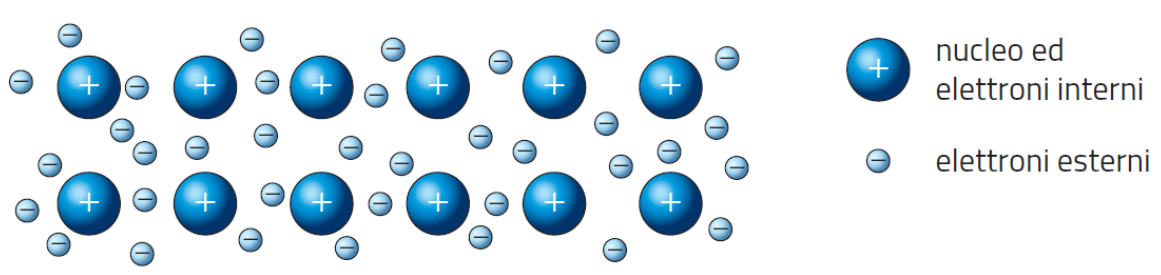
\includegraphics[width=12cm]{immagini/legame-metallico.png}
\end{figure}

Nei metalli gli atomi occupano posizioni ben definite all'interno di una struttura cristallina. A differenza dei composti ionici però qua non possiamo parlare di ioni: gli atomi sono neutri, solo che i loro elettroni esterni occupano una banda e non più un livello. Finora infatti abbiamo parlato di energie ben precise per gli orbitali, ma non è più così all'interno di una banda, o per meglio dire l'energia dei singoli livelli continua ad esserci, ma poiché essi sono in numero elevato, possiamo immaginare che la differenza in energia tra un livello energetico e il successivo sia piccolissima, al punto tale da immaginare non più l'esistenza di orbitali con energie nette e separate, ma una banda all'interno della quale l'elettrone possa muoversi

\subsection{Esempi vari}
Nei vari esempi che seguono, per razionalizzare i i valori sperimentali dei momenti di dipolo, ragioneremo sulla direzionalità dei legami e sulla differenza di elettronegatività degli atomi coinvolti.

\vspace{0.2cm}$\bullet$ ES1 F$_2$

\begin{figure}[htp]
    \centering
    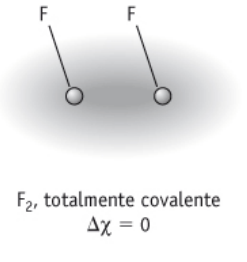
\includegraphics[width=4cm]{immagini/F_2.png}
\end{figure}

Due atomi di fluoro formano la molecola F$_2$. Sebbene il fluoro sia estremamente negativo, i due atomi sono uguali, per cui la differenza in elettronegatività è pari a zero, quindi la condivisione dei due elettroni di legame è totale e il sistema è covalente.

\vspace{0.2cm}$\bullet$ ES2 HF

\begin{figure}[htp]
    \centering
    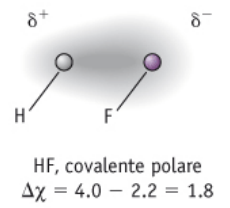
\includegraphics[width=5cm]{immagini/HF.png}
\end{figure}
Nell'acido fluoridrico la differenza di elettronegatività tra i due atomi è cospicua, e infatti la carica di legame(che può essere immaginata come una nube elettronica che circonda i due atomi) sarà più spostata verso l'atomo di fluoro e quindi meno presente sull'idrogeno. Il legame sarà allora covalente polare, con una parziale carica negativa $\delta^-$ sul fluoro e una parziale carica positiva $\delta^+$ sull'idrogeno. 

\vspace{0.2cm}$\bullet$ ES3 LiF

\begin{figure}[htp]
    \centering
    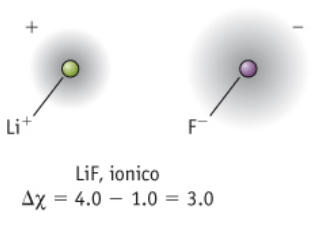
\includegraphics[width=5cm]{immagini/LiF.png}
\end{figure}

\vspace{-0.4cm}In un sistema come il fluoruro di litio, la differenza di elettronegatività è elevata, per cui non ci sarà la nube continua tra i due atomi.

Per questi sistemi si immagina che si abbia una cessione di elettroni, per cui non avremo Li e F ma Li$^+$ e F$^-$, cioè è come se il litio avesse ceduto il suo elettrone di valenza al fluoro, il quale tralaltro acquistandolo avrà la configurazione elettronica esterna dei gas nobili.
Un sistema siffatto è etichettato sistema ionico.

\vspace{0.2cm}$\bullet$ ES4 HCl

\vspace{-0.4cm}\begin{figure}[htp]
    \centering
    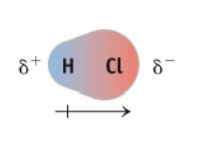
\includegraphics[width=5cm]{immagini/HCl.png}
\end{figure}

\vspace{-0.4cm}Nell'acido cloridrico la differenza di elettronegatività tra idrogeno e cloro è abbastanza evidente, per cui il legame è covalente polare.

Dato che stiamo ipotizzando che su tale molecola ci sia una buona polarità, come conseguenza ci aspettiamo un momento di dipolo.
Per verificarne l'esistenza basta mettere dell'HCl gassoso in un contenitore dove presenti le espansioni polari di un elettromagnete. Se il campo elettrico è nullo, l'orientazione delle molecole sarà casuale; se invece applichiamo una differenza di potenziale tra le due piastre osserveremo che le molecole si orientano in modo tale che il cloro sia rivolto verso la lamina positiva (a potenziale maggiore).
\begin{figure}[htp]
    \centering
    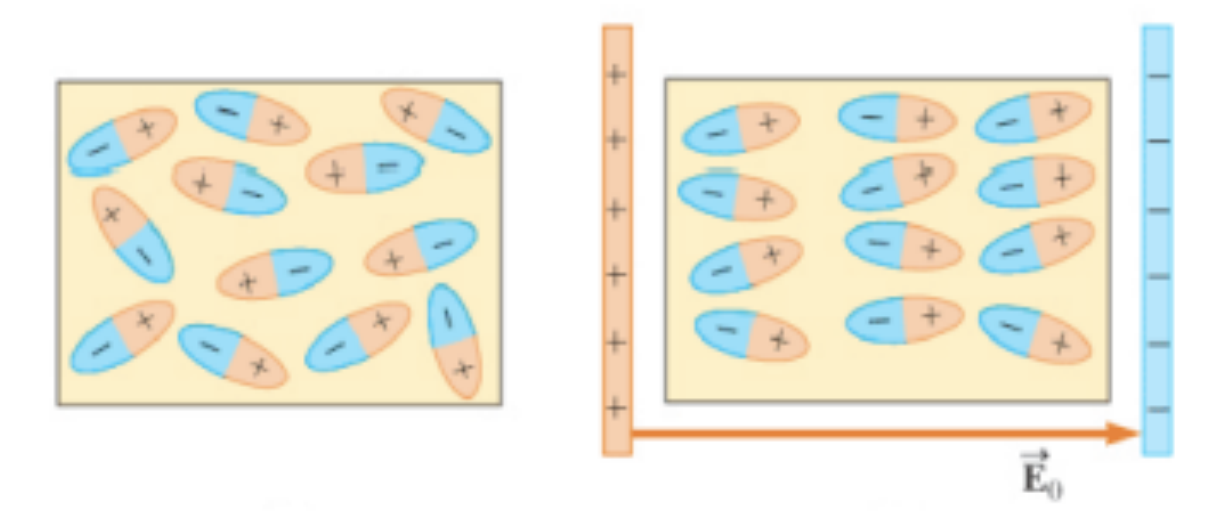
\includegraphics[width=10cm]{immagini/condensatore.png}
\end{figure}
Come facciamo ad accorgercene?
Il sistema che si viene così a costituire è un condensatore, dove tra le armature anziché il vuoto c'è un dielettrico: l'HCl. In questo modo possiamo quindi misurare il momento di dipolo, la cui unità di misura nel SI è il Coulomb per metro, con cui le molecole danno dei valori dell'ordine di 10$^{-30}$, per cui si una un'altra unità di misura che è il Debye (D). Vale la relazione:
$$1D=3.336\cdot10^{-30}$$
Per l'acido cloridrico si misura un momento di dipolo pari a 1.03 D.

\vspace{0.2cm}$\bullet$ ES5 CO$_2$

\hspace{0.5cm}\begin{minipage}{0.2\textwidth}
    \begin{figure}[H]
    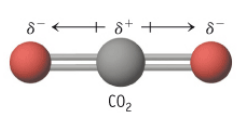
\includegraphics[width=4cm]{immagini/CO_2.png}
    \end{figure}
    \end{minipage} \hfill
    \begin{minipage}{0.65\textwidth}
    \vspace{0.4cm}Descrivendo l'anidride carbonica col formalismo di Lewis notavamo che sul carbonio non ci sono coppie solitarie, perché raggiunge l'ottetto grazie ai due doppi legami carbonio-ossigeno, mentre su ciascun ossigeno ce ne sono due. La geometria che tiene più lontani gli i due atommi di ossigeno con le coppie di elettroni rimaste è quella lineare.
    
    La differenza in elettronegatività tra carbonio e ossigeno è cospicua, quindi singolarmente troviamo un momento di dipolo nei due diversi legami, ma questi si annullano a vicenda perché sono uguali in modulo ma opposti in verso. Pertanto questa molecola ha un momento di dipolo netto pari a zero, cioè non è polare, pur essendo polari i singoli legami.
    \end{minipage}

\vspace{0.2cm}$\bullet$ ES6 H$_2$O

\hspace{0.5cm}\begin{minipage}{0.2\textwidth}
    \begin{figure}[H]
    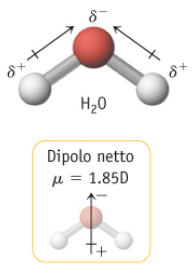
\includegraphics[width=3cm]{immagini/H_2O.png}
    \end{figure}
    \end{minipage} \hfill
    \begin{minipage}{0.65\textwidth}
    \vspace{0.6cm}Descrivendo l'acqua col formalismo di Lewis notavamo due coppie solitarie sull'ossigeno. Dovendo ragionare su un sistema con 4 coppie di elettroni usiamo l'idea del sistema tetraedrico nel quale però le due coppie solitarie stringono il legame, che avrà un angolo di 104.5°. Considerando solo gli atomi, questa molecola sarà piana ma angolata.

    La differenza in elettronegatività tra idrogeno e ossigeno è cospicua, per cui entrambi i legami mostreranno un momento di dipolo. In questo caso però, a causa della geometria molecolare, la loro composizione dà luogo ad un momento di dipolo netto pari a 1.85D. Grazie ad esso l'acqua è la molecola che permette la vita.    
    \end{minipage}

\vspace{0.2cm}$\bullet$ ES7 BF$_3$

\begin{figure}[htp]
    \centering
    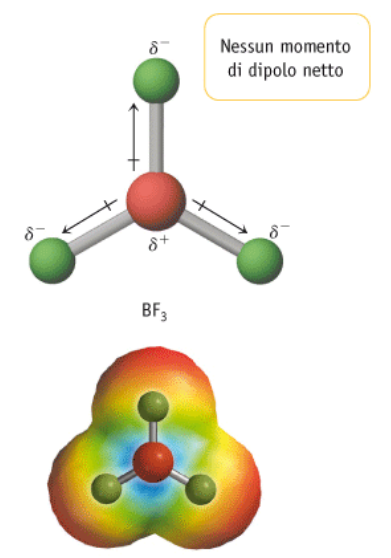
\includegraphics[width=8cm]{immagini/BF_3-dipolo.png}
\end{figure}

Nel descrivere tale molecola abbiamo detto che il boro presenta ibridizzazione sp$^2$, per cui essa sarà una molecola planare con angoli di 120°.

Il fluoro è parecchio più elettronegativo del boro, quindi ciascun legame mostrerà polarità, con la carica di legame addensata sul fluoro.

Essendo planare, la composizione dei tre momenti di dipolo, fra loro uguali in modulo, dà un momento di dipolo netto pari a zero, per cui il BF$_3$ non ha polarità. 

\vspace{0.2cm}$\bullet$ ES8 Cl$_2$CO

\begin{figure}[htp]
    \centering
    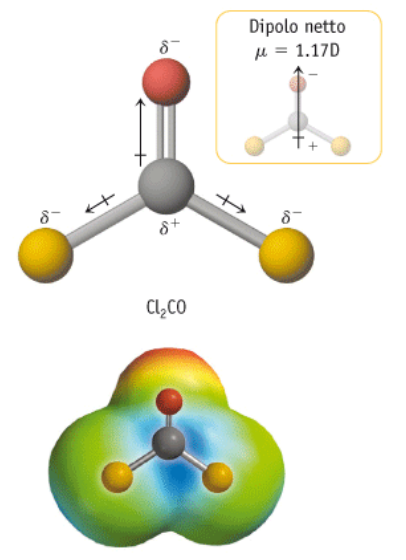
\includegraphics[width=8cm]{immagini/Cl_2CO.png}
\end{figure}

Nel fosgene un atomo di carbonio centrale è legato all'ossigeno tramite un doppio legame e a due atomi di cloro tramite due legami semplici. Sia il cloro che l'ossigeno sono parecchio più elettronegativi del carbonio, quindi ciascun legame mostrerà polarità con la freccia rivolta verso gli atomi esterni. Il momento di dipolo del legame carbonio-ossigeno è più forte, per cui la composizione darà un momento di dipolo netto pari a 1.17D.

\vspace{0.2cm}$\bullet$ ES9 NH$_3$

\begin{figure}[htp]
    \centering
    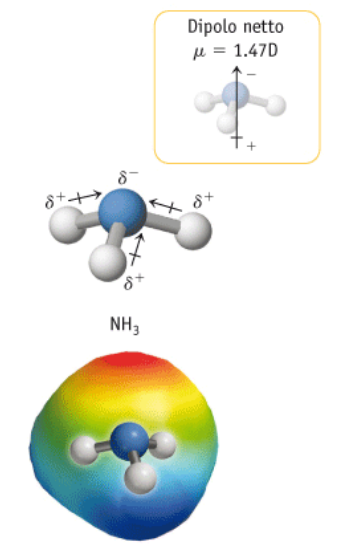
\includegraphics[width=8cm]{immagini/NH_3.png}
\end{figure}

Nell'ammoniaca è l'azoto centrale ad essere più elettronegativo, e lo è parecchio rispetto all'idrogeno. Ne segue che ogni legame mosterà polarità la cui freccia è rivolta verso questo. Inoltre col formalismo di Lewis abbiamo visto che su di esso è presente una coppia solitaria, la quale lo solleva dal piano dei tre atomi di idrogeno, per cui il momento di dipolo netto sarà diverso da zero.

Se non ci fosse stata la coppia solitaria, l'azoto si sarebbe disposto nel piano individuato dai 3 idrogeni come nel baso del \ce{BF_3} e quindi non si avrebbe avuto un momento di dipolo netto.

\vspace{0.2cm}$\bullet$ ES10 CH$_4$

\hspace{0.5cm}\begin{minipage}{0.2\textwidth}
\begin{figure}[H]
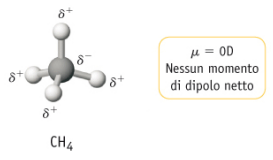
\includegraphics[width=5cm]{immagini/CH_4.png}
\end{figure}
\end{minipage} \hfill
\begin{minipage}{0.5\textwidth}
 Nel metano c'è una buona differenza in elettronegatività tra carbonio e idrogeno, ma a causa della sua geometria tetraedrica la risultante dei momenti di dipolo, uno per ciascun legame, sia pari a zero. Nei fatti il momento di dipolo osservato è zero.
\end{minipage}

\vspace{0.2cm}$\bullet$ ES11 CH$_3$Cl

\hspace{0.5cm}\begin{minipage}{0.2\textwidth}
\begin{figure}[H]
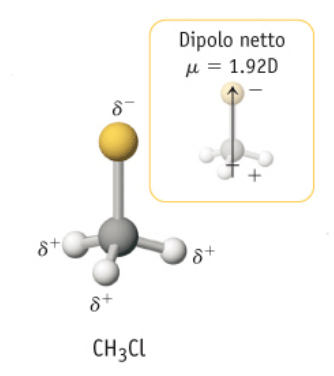
\includegraphics[width=5cm]{immagini/CH_3Cl.png}
\end{figure}
\end{minipage} \hfill
\begin{minipage}{0.5\textwidth}
\vspace{0.4cm}Se nel metano sostituiamo un idrogeno qualunque con un atomo di cloro, la molecola così ottenuta mostra un momento di dipolo netto. Il motivo è che il momento di dipolo del legame cloro-carbonio non è più equivalente agli altri tre, per cui nella loro composizione non si annullano a vicenda.
\end{minipage}

\vspace{0.2cm}$\bullet$ ES12 CH$_2$Cl$_2$

\hspace{0.5cm}\begin{minipage}{0.2\textwidth}
\begin{figure}[H]
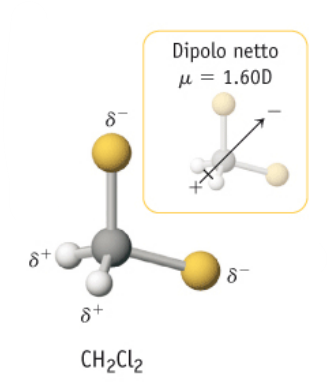
\includegraphics[width=5cm]{immagini/CH_2Cl_2.png}
\end{figure}
\end{minipage} \hfill
\begin{minipage}{0.5\textwidth}
Se sostituiamo un secondo idrogeno con un altro atomo di cloro, la composizione dei momenti di dipolo ne darà uno netto ancora diverso da zero, sebbene minore rispetto al caso precedente.
\end{minipage}

\vspace{0.2cm}$\bullet$ ES13 CHCl$_3$

\hspace{0.5cm}\begin{minipage}{0.2\textwidth}
\begin{figure}[H]
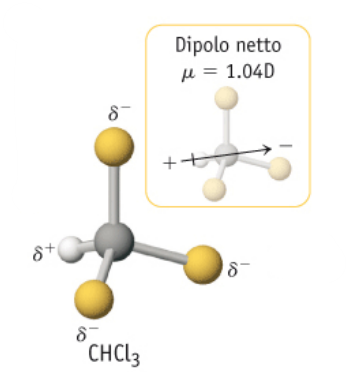
\includegraphics[width=5cm]{immagini/CHCl_3.png}
\end{figure}
\end{minipage} \hfill
\begin{minipage}{0.5\textwidth}
Sostituendo anche un terzo idrogeno con un ulteriore atomo di cloro, la composizione dei momenti di dipolo sarà anche stavolta diversa da zero, ma ancora più piccola.
\end{minipage}

\vspace{0.2cm}$\bullet$ ES14 CCl$_4$

\hspace{0.5cm}\begin{minipage}{0.2\textwidth}
\begin{figure}[H]
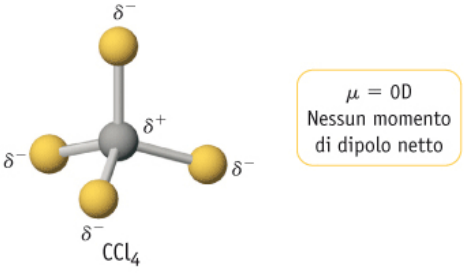
\includegraphics[width=5cm]{immagini/CCl_4.png}
\end{figure}
\end{minipage} \hfill
\begin{minipage}{0.5\textwidth}
Nel momento in cui anche il quarto e ultimo idrogeno viene sostituito con un atomo di cloro otteniamo il tetracloruro di carbonio, il cui sistema sarà di nuovo simmetrico. Per esso la composizione dei momenti di dipolo sarà pari a zero, fatto confermato dalle evidenze sperimentali.
\end{minipage}


\vspace{0.2cm}$\bullet$ ES15 L'ordine di legame
\begin{figure}[htp]
    \centering
    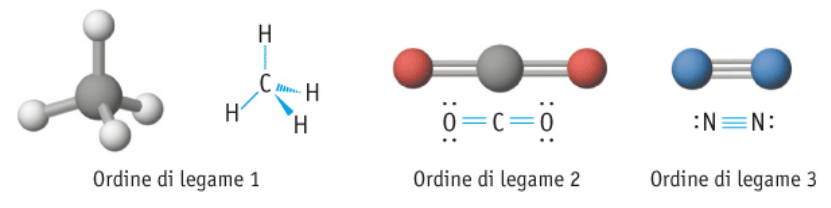
\includegraphics[width=14cm]{immagini/ordine-di-legame.png}
\end{figure}

Consideriamo queste molecole, in modo da dare nuovamente il cocnetto di ordine di legame. Diremo che un legame semplice ha ordine di legame 1, uno doppio ordine di legame 2 e uno triplo ordine di legame 3. Tuttavia nell'istante in cui ci fossero sistemi per i quali qualche doppio legame si possa ripartire su più legami semplici l'ordine non era più intero, ma frazionario
\subsection{Il legame ionico}
in esso la dislocazione delle cariche e totale, per cui immaginiamo che ci sia cessione dell'elettrone e in conseguenza a ciò si formino uno ione positivo e uno negativo.

\subsection{Considerazioni energetiche nella formazione di un legame ionico}
Immaginiamo di avere due atomi separati, ad esempio litio e fluoro.

Nella specie LiF sappiamo da altri studi che effettivamente si hanno ioni litio e fluoruro, ossia il litio ha ceduto il suo unico elettrone esterno al fluoro.

Se il litio cede un elettrone, vuol dire che è stata spesa dell'energia per strapparglielo, per esattezza si deve spendere una energia pari a quella di prima ionizzazione del litio, che ammonta a 520 kJ/mol.
Al contempo, poiché il fluoro sta acquistando un elettrone, dovrà emettere una certa quantità di energia pari alla sua affinità elettronica, che vale -328 kJ/mol. Questo significa che essa da sola non basta a ionizzare il litio, ossia se mettessimo vicini ma isolati due atomi, uno di fluoro e uno di litio, non si formerebbero questi ioni, in quanto il fluoro tenderebbe a catturare l'elettrone del litio, ma libererebbe un'energia non sufficiente a ionizzare il litio, poiché tale processo richiede più energia.

Ne segue che questi due atomi isolati non daranno luogo alla specie molecolare Li$^+$F$^-$.

Considerazioni analoghe valgono per qualsiasi altro composto ionico, come ad esempio l'NaCl: l'affinità elettrica del cloro non è sufficiente a strappare l'elettrone al sodio affinché diventi Na$^+$, in quanto il suo potenziale di prima ionizzazione è più altro dell'affinità elettronica del cloro, per cui la molecola NaCl non può esistere come singola entità.

Tuttavia sia il fluoruro di litio, che il cloruro di sodio, esistono.

Dobbiamo quindi trovare la fonte di questo legame, cioè capire perché esiste il solido ma non la molecola singola.

La prima domanda che quindi ci poniamo è: "Dove sta la forza che tiene legati insieme questi ioni, dato che il sistema solido esiste?"

Una prima risposta è che essa deve stare nella struttura adottata in fase solida. È lì che dobbiamo cercare la ragione, perché se la molecola non esiste e il solido si è chiaro che in quest'ultimo ci sarà un qualche contributo in energia che permette la formazione della specie chimica.

Per mostrare la validità di tale ipotesi utilizziamo un ciclo termodinamico, chiamato "\textbf{Ciclo di Born-Haber}", che permette di razionalizzare la ragione dell'esistenza dei solidi di tutti i sistemi ionici.

Il nostro obiettivo è capire perché possiamo prendere del litio solido Li$_{(s)}$, aggiungere del fluoro gassoso F$_{(g)}$ e ottenere il fluoruro di litio solido LiF$_{(s)}$ senza problemi.

Sappiamo però che il fluoruro di litio presenta una struttura solida nella quale ioni litio e ioni fluoruro occupano precise posizioni reticolari, quindi non è una struttura disordinata, anzi è estremamente ordinata.

L'energia che stiamo cercando è la variazione di entalpia che si ha nella formazione del solido ionico a seguito della reazione:
$$\ce{Li^{+}_{(g)} + F^{-}_{(g)} -> LiF_{(s)}} \quad \Delta\text{H=?}$$
In questa reazione una mole di litio gassoso reagisce con una mole di fluoro gassoso per dare luogo ad una mole di fluoruro di litio solido, in quanto non esiste in forma gassosa.

Purtroppo questa reazione è impossibile da realizzare perché in natura non abbiamo né ioni litio gassosi, in quanto in litio è presente solo come composto insieme a qualche altro elemento, né ioni fluoruro gassosi, in quanto esiste in forma molecolare F$_2$, per cui non possiamo partire da questi reagenti.

Quello che possiamo fare è partire dai composti del litio, fonderli, fare elettrolisi e ridurre il Li$^+$ a Li$^0$ tramite processi elettrochimici. Dopodiché facciamo reagire questo insieme al fluoro gassoso e otteniamo:
$$\ce{Li_{(s)} + \frac{1}{2}F_{2(g)} -> LiF_{(s)}}$$
Notiamo che questa reazione è diversa da quella di partenza, ma se stiamo attenti a lavorare a pressione costante, le energie scambiate diventano variazioni di entalpia $\Delta$H, che è una funzione di stato, per cui non dipenderà dal particolare percorso, ma solo da stato iniziale e finale. In altre parole possiamo fare avvenire questa reazione tramite il percorso diretto o tramite il percorso più complesso, contenuto all'interno del ciclo di Born-Haber, e la variazione di energia che si ha passando da reagenti a prodotti sarà la stessa.

Il processo che si usa è il seguente:
\begin{itemize}
    \item Si parte dal litio solido e si spende una certa energia $\Delta\text{H}_{atomiz}$ per portarlo in fase gassosa che chiamiamo energia di atomizzazione o evaporazione del litio, facilmente misurabile con un calorimetro.
    \item Si rompe la molecola biatomica del fluoro, passando così da F$_2$ a 2F. L'energia così spesa è quella di dissociazione del fluoro che è detta binding energy (BE). Poiché ci serve solo un atomo di fluoro e da ogni molecola ne otteniamo due, ci basta metà di questa energia.
    
    A questo punto avremo litio e fluoro entrambi allo stato gassoso.
    \item Si fornisce l'energia di prima ionizzazione $IP_1$ del litio per ottenere il suo catione:
    
    \ce{Li_{(g)} -> Li^{+}_{(g)} + 1e}
    \item L'elettrone ottenuto dalla ionizzazione del litio viene acquistato dal fluoro, il quale diventa F$^-$ e cede un'energia pari alla sua affinità elettronica $EA$.
    \item Arriviamo così ad avere ioni $Li^+$ e $F^-$ gassosi, che sono i reagenti della reazione considerata inizialmente, la quale ci interessa poiché in essa vi è tutta la stabilità del sistema solido.
    
    Essi insieme daranno luogo al fluoruro di litio solido e quindi pur non avendo fatto il percorso diretto siamo arrivati allo stesso prodotto:
\end{itemize}

\begin{figure}[htp]
    \centering
    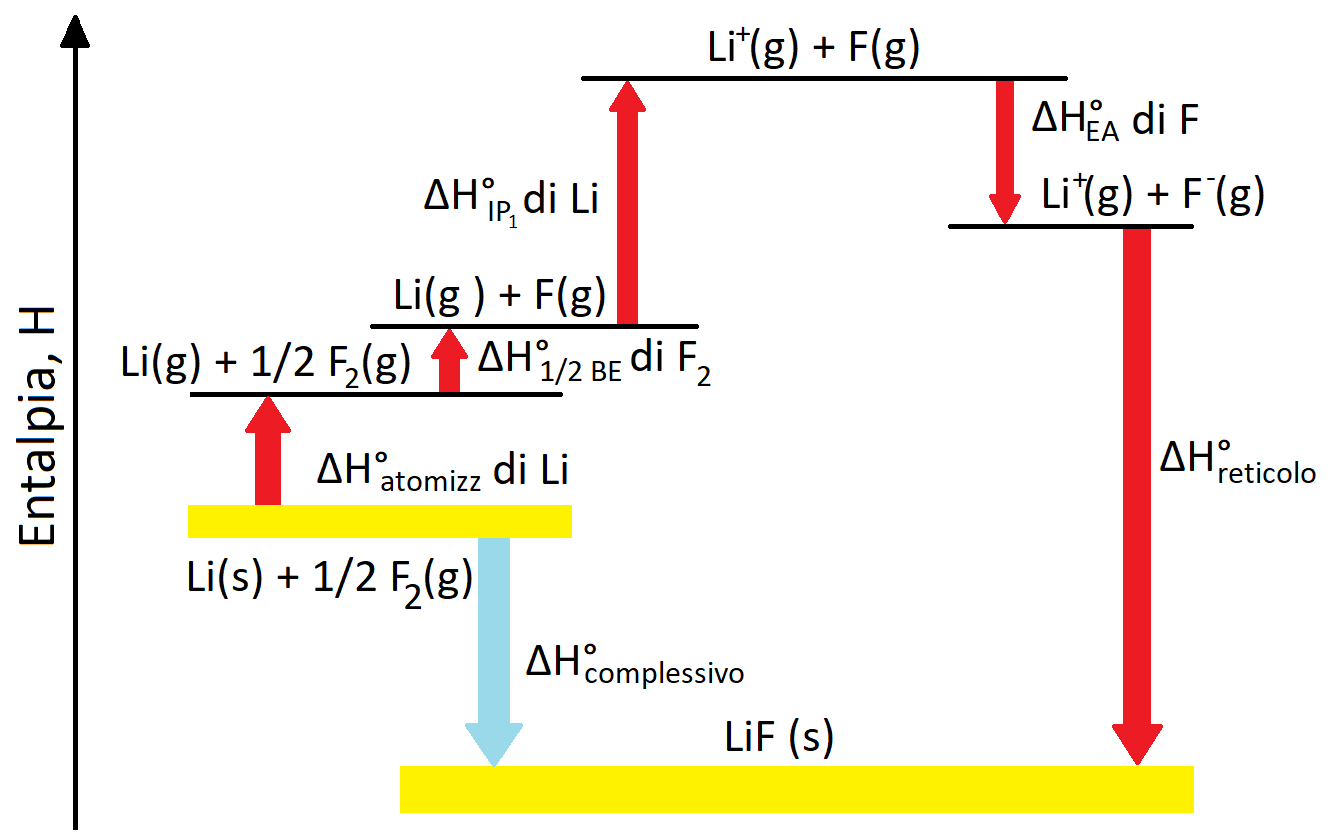
\includegraphics[width=10cm]{immagini/Ciclo-Born-Haber.png}
\end{figure}

Poiché stato iniziale e stato finale sono gli stessi, la somma di tutti questi calori deve essere uguale al calore scambiato nel percorso diretto.

Il calore di formazione emesso nel processo diretto lo sappiamo calcolare, mentre nel processo complesso non sappiamo misurare solo il calore emesso per passare dagli ioni gassosi al reticolo solido, la quale però può essere calcolata facendo la differenza tra valori sperimentali:
$$\Delta\rm{H}_{reticolo}=\Delta\rm{H}_{complessivo} - \Delta\rm{H}_{atomiz} - \Delta\rm{H}_{BE} - \Delta\rm{H}_{IP_1} + \Delta\rm{H}_{EA}$$
Si trova che, alla temperatura di 25° C e alla pressione di 1 bar, il $\Delta\rm{H}$ complessivo è pari a -617 kJ/mol. È negativo perché quando mettiamo insieme litio e fluoro spontaneamente si forma il fluoruro di litio, emettendo tale calore.

Facendo la differenza tra tale calore e gli altri calori misurabili si trova che l'energia di reticolo vale -1050 kJ/mol, che viene emessa con la formazione del reticolo.

Quindi il legame chimico nei sistemi ionici sta tutto nella formazione del reticolo, cioè la stabilità del solido e la inesistenza della singola molecola sta nel fatto che in questa l'energia emessa dal fluoro quando acquista un elettrone non basta a ionizzare il litio, che è quello che dovrebbe cedere l'elettrone, per cui la molecola non potrà formarsi, mentre quando si forma il solido questi ioni liberano una grande quantità di energia, cosa che permette al solido di formarsi. Quindi è proprio all'interno del reticolo che si trova la stabilità di questo sistema: quando questi ioni vanno ad occupare precise posizioni reticolari si forma questo reticolo estremamente stabile con l'emissione di una quantità molto grande di energia.

Questo discorso vale per tutti i solidi ionici: non esistendo le loro molecole ma il loro solido si, vuol dire che la stabilità è conferita dall'arrangiamento in fase solida.

\vspace{0.2cm}\textbf{Legge di Hess}: il calore scambiato a pressione costante in una reazione chimica che possa essere scomposta in più reazioni parziali è indipendente dagli stati intermedi attraverso i quali si evolve il sistema e dipende solo dagli stati iniziale e finale. La variazione di calore è pari alla somma algebrica delle variazioni di calore dei singoli stadi.

A causa di tale legge, se abbiamo calori scambiati a pressione costante il sistema può essere rappresentato attraverso una serie di stati intermedi, ottenendo così un ciclo termodinamico e quindi le energie coinvolte dipendono solo dallo stato iniziale e da quello finale.

\vspace{0.2cm}N.B.: Se chiede di parlare del legame ionico attraverso un modello termodinamico descrivi il ciclo, ma se chiede perché abbiamo la necessità di usare il ciclo, il motivo è perché siamo interessati al $\Delta\rm{H}_{reticolo}$, che è l'energia del reticolo cristallino, perché in tale reazione da un lato abbiamo gli ioni gassosi e dall'altro li abbiamo nel solido, nel reticolo cristallino, per cui vogliamo conoscere l'energia che viene emessa quando questo si forma, ossia partiamo da un'energia molto alta di questi ioni $Li^+$ e $F^-$ gassosi e quando questi si uniscono per formare il solido emettono una quantità enorme di energia, e il sistema si stabilizza tantissimo. Questa energia emessa si chiama "energia reticolare" perché è l'energia del reticolo. Quindi in questo secondo caso la prima cosa da dire è:"l'energia reticolare è l'energia associata al processo nel quale sono reagenti, in questo caso particolare, ione litio gassoso più ione fluoruro gassoso, e il prodotto è il fluoruro di litio, ma noi non siamo in grado di effettuare questa reazioni, perché questi reagenti non li abbiamo. Ecco perché usiamo il ciclo di Born-Haber, il quale mi permette di aggirare questo problema". Dopodiché si  inizia a parlare del ciclo, quindi diamo la motivazione (voler conoscere l'energia del reticolo, che è quella che tiene insieme gli ioni nel reticolo).

\subsection{Differenze tra composti molecolari e composti ionici}
Per i composti molecolari esistono le singole molecole, per quelli ionici no: essi esistono solo in forma di reticolo cristallino, dove gli ioni occupano posizioni ben precise, alternandosi, in tutte e 3 le direzioni.

La conseguenza di ciò è che se mettiamo in acqua ad esempio il glucosio \ce{C_6H_{12}O_6}, che è un composto molecolare, esso resta tale, mentre se mettiamo ad esempio il cloruro di sodio NaCl esso si dissocia in ioni Na$^+$ e Cl$^-$. Ciò che avviene è che l'acqua aggredisce il cristallo e stacca singoli ioni, i quali vengono portati in soluzione con delle molecole di acqua che li circondano. In particolare gli ioni positivi saranno circondati dagli atomi di ossigeno dell'acqua, in quanto essi reagiranno con la parziale carica negativa presente su questo, mentre gli ioni negativi saranno, mentre gli ioni negativi saranno circondati dagli idrogeni dell'acqua poiché interagiranno con la parziale carica positiva presente su questi:
\begin{figure}[htp]
    \centering
    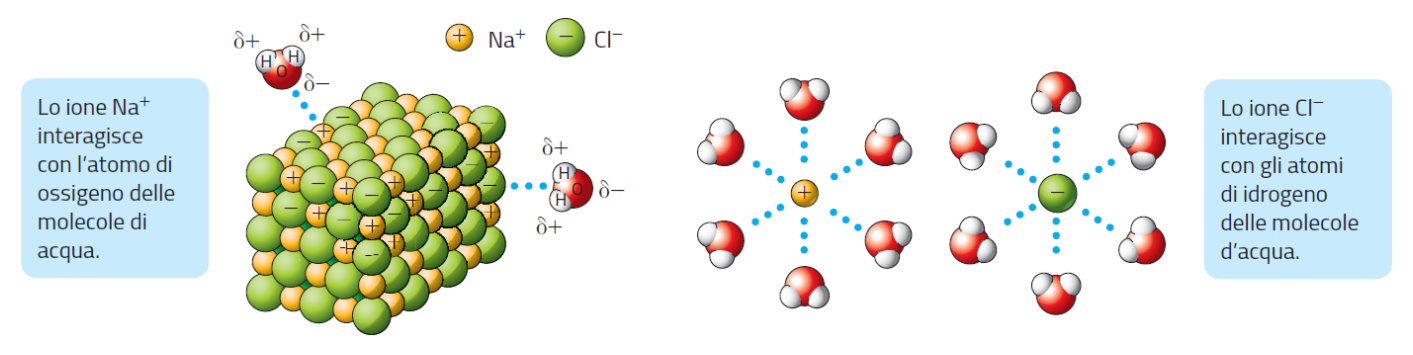
\includegraphics[width=15cm]{immagini/interazione-acqua-ioni.png}
\end{figure}
Dunque in soluzione si avranno ioni.

L'evidenza sperimentale di tale fatto si ottiene confrontando tre circuiti elettrici con una lampadina, dove in uno inseriamo in serie dell'NaCl solido, in un altro dell'NaCl fuso e in un terzo una soluzione di NaCl sciolto in acqua. Il primo non permette la conduzione (la lampada non si accende), il secondo permette una leggera conduzione (la lampada si accende ma la luce è fioca), il terzo permette una grande conduzione (la lampada si accende con luminosità maggiore).

\begin{figure}[htp]
    \centering
    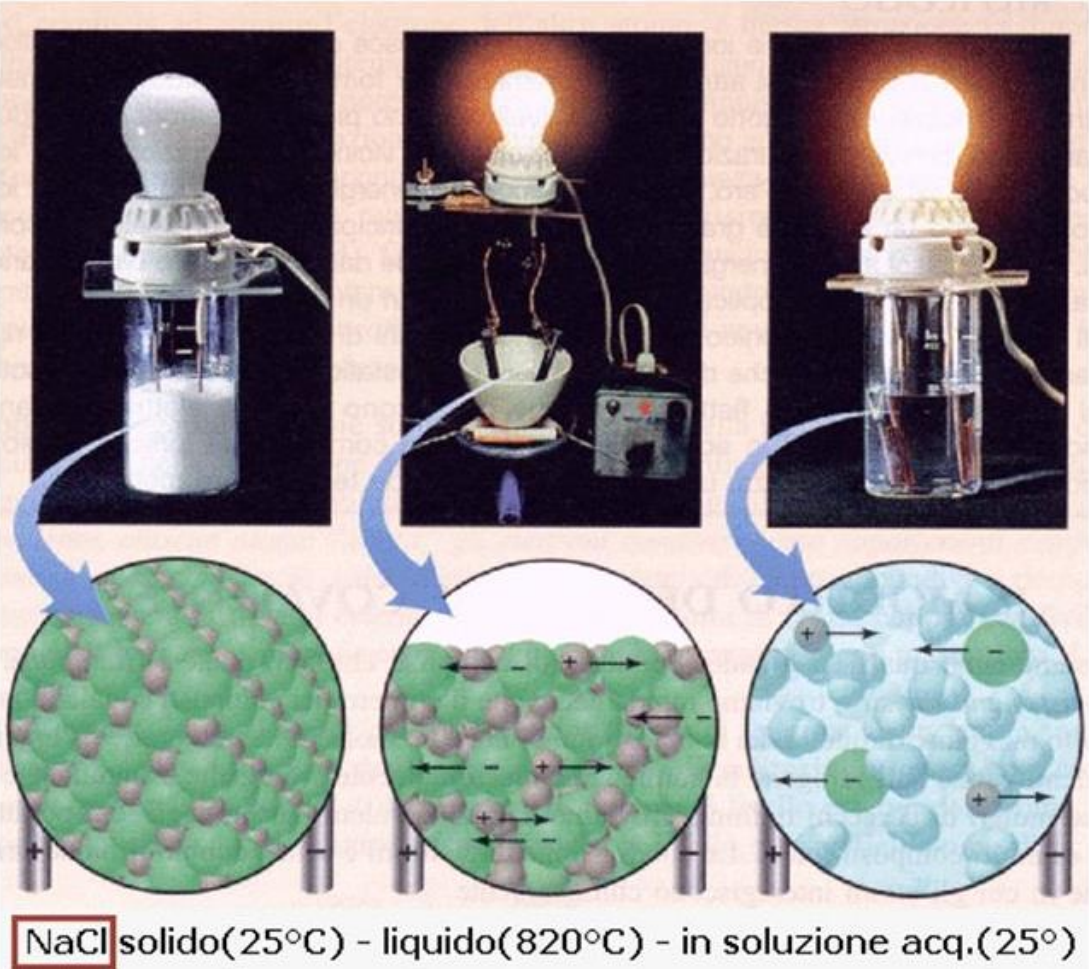
\includegraphics[width=10cm]{immagini/lampadina.png}
\end{figure}

Tale esperimento mostra l'esistenza degli ioni, che sono i portatori di carica che permettono la conduzione.

Se invece avessimo collegato a lampadina ad una soluzione acquosa contenente zucchero, la lampadina non si accenderebbe. Il motivo è che lo zucchero è un composto molecolare, per cui non si scioglie in acqua e non dà origine a ioni.
\subsection{Proprietà fisiche dei composti ionici}
Tipicamente i composti ionici sono duri, rigidi e fragili, cioè è facile romperli.

Se solidi, non conducono elettricità, per cui costituiscono dei buoni isolanti. Se invece li portiamo a fusione (che per tali composti significa portarli ad una temperatura di 800-1000°C) iniziano a condurre. Se invece li sciogliamo in acqua la mobilità degli ioni diventa elevata e la conducibilità è ancora maggiore. Tale fatto è la dimostrazione dell'esistenza degli ioni come portatori di carica.

In genere hanno temperature di fusione elevate, perché dobbiamo abbattere l'energia reticolare, che è molto elevata, per poter liberare gli ioni dal reticolo.

All'interno dei reticoli gli ioni sono disposti alternatamente nelle varie direzioni
\begin{figure}[htp]
    \centering
    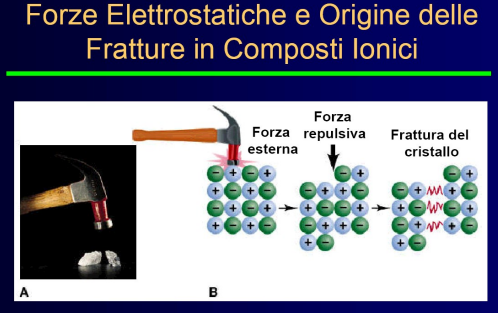
\includegraphics[width=10cm]{immagini/struttura-composti-ionici.png}
\end{figure}
Immaginiamo un sistema bidimensionale. Se cerchiamo di rompere il cristallo, lo si deve spezzare e far scivolare il sistema in un piano. Se riusciamo a fare ciò, riusciamo a rompere il cristallo.
\subsection{Il modello del legame covalente}
Consideriamo due atomi di idrogeno, che immaginiamo inizialmente posti a distanza infinita, i quali via via si avvicinano. Nella situazione iniziale possiamo dire che non esiste alcuna interazione fra i due atomi, ma nell'istante in cui la distanza, pur grandissima che sia ma comunque finita, i due atomi iniziano ad interagire.

Il grafico dell'energia potenziale ha il seguente andamento:

\begin{figure}[htp]
    \centering
    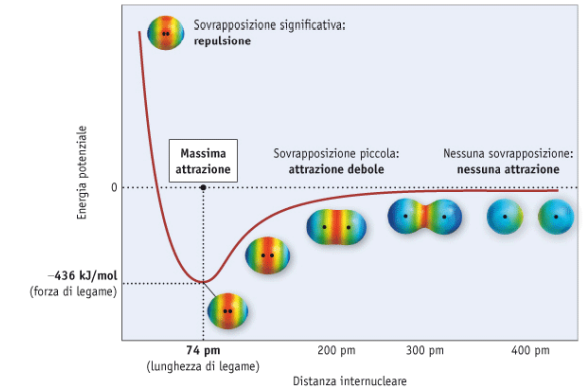
\includegraphics[width=10cm]{immagini/energia-potenziale.png}
\end{figure}

Essa sarà l'energia di due atomi di idrogeno che si avvicinano.

Inizialmente abbiamo valori di energia prossimi a zero, ossia quando la distanza è infinita questo sistema ha energia potenziale nulla. Nell'istante in cui la distanza diventa misurabile i due atomi iniziano ad interagire. Ciò significa che quando i due atomi si avvicinano si può già parlare di energia negativa e quindi i due atomi si stanno realmente legando, ossia possiamo immaginare che si inizi ad instaurare un legame chimico.

I due atomi si avvicineranno fino ad una certa distanza in cui si ha il minimo di energia per il sistema. Per due atomi di idrogeno legati si ottiene quando la distanza di equilibrio (perché i due atomi vibrano, non sono rigidamente fermi) è pari 0.74 Å.

Se tentassimo di avvicinarli ulteriormente, l'energia inizierebbe a crescere velocemente superando persino lo zero, perché inizia ad essere incisiva la repulsione tra i nuclei e tra gli elettroni. Se invece li allontanassimo l'energia tenderebbe al valore U=0, che prende il nome di "asintoto di dissociazione", e i due atomi non sarebbbero più legati.

Nel punto di minimo di energia per due atomi di idrogeno si trova un valore di -436 kJ/mol, che è il valore di energia che dovremmo spendere per rompere il legame della molecola H$_2$.

\vspace{0.2cm}
Seguendo questa curva sembrerebbe che siano possibili tutte le energie, ma non è così. Infatti abbiamo detto che l'energia è quantizzata, e tale è anche l'energia di vibrazione di due atomi di idrogeno all'interno di una molecola di H$_2$, per cui solo alcuni dei valori rappresentati sono permessi. Questo modo di rappresentare l'energia è più adatto per un sistema macroscopicom i cui valori di energia non siano quantizzati. Tuttavia si usa comunque questa rappresentazione per sistemi quantizzati, dato che i valori possibili di energia stanno su questa curva.
\begin{figure}[htp]
    \centering
    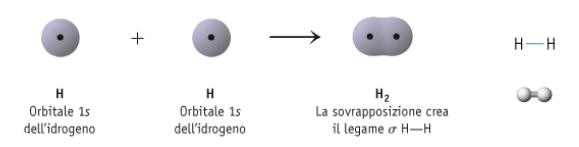
\includegraphics[width=10cm]{immagini/legame-H_2.png}
\end{figure}

Quello che quindi stiamo immaginando è di avere due atomi di idrogeno con due orbitali 1s, ciascuno con un proprio elettroni. Questi due orbitali interagiscono dra di loro per dar luogo alla formazione di un legame chimico, con l'ottenimento della molecola H$_2$. Se abbiamo due orbitali di tipo $s$, cioè a simmetria sferica, si ottiene un legame di tipo $\sigma$, che è quello che rappresentiamo come una lineetta tra i due atomi di idrogeno. 

\vspace{0.2cm}Consideriamo adesso l'acido fluoridrico HF. Il fluoro è il primo degli alogeni. Ha orbitali 2s e 2p come orbitali di valenza. L'orbitale 2s è parecchio interno come energia, quindi non adatto per interagire con l'orbitale 1s dell'atomo di idrogeno. Abbiamo poi i tre orbitali $p$: uno di questi avrà i suoi lobi orientati lungo quello che etichettiamo "asse di legame". L'orbitale p del fluoro orientato lungo tale asse, interagirà con l'orbitale 1s dell'idrogeno e formerà un legame $\sigma$, perché si ha sovrapposizione lungo l'asse di legame, sebbene gli orbitali interagenti siano uno di tipo $s$ e uno di tipo $p$
\begin{figure}[htp]
    \centering
    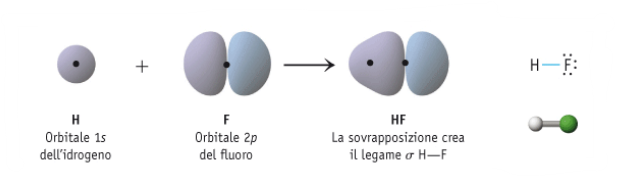
\includegraphics[width=10cm]{immagini/legame_H-F.png}
\end{figure}

Va da notare che i due lobi dell'orbitale p hanno colori diversi, e ad interagire con l'orbitale s dell'idrogeno è quello che ha lo stesso colore di ques'ultimo. Il motivo è che i lobi degli orbitali p hanno segno opposto, pertanto affinché i due orbitali interagiscano si deve scegliere il lobo avente lo stesso segno.

\vspace{0.2cm} Prendiamo adesso in esame la molecola F$_2$. Essendo due atomi identici avranno gli stessi orbitali, e in particolare quelli più esterni nel fluoro sono i $p$. Per ciascun atomo di fluoro, uno dei tre giacerà lungo l'asse di legame:
\begin{figure}[htp]
    \centering
    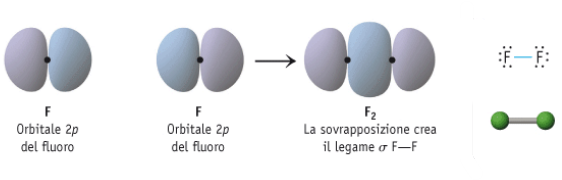
\includegraphics[width=10cm]{immagini/legame-F_2.png}
\end{figure}

Se li orientiamo in modo tale che i lobi che si affacciano l'uno sull'altro abbiano lo stesso segno ancora una volta otterremo un orbitale $\sigma$, in quanto ci sarà addensamento lungo la congiungente i due nuclei cioè lungo l'asse di legame, nonostante esso si stia formando tramite due orbitali $p$.

\vspace{0.2cm} Da questi esempi deduciamo che il legame $\sigma$ non necessariamente debba venir fuori da due orbitali di tipo s, ma può venir fuori anche un orbitale $s$ e uno $p$ o da due orbitali $p$. La cosa fondamentale è che gli orbitali che interagiscono siano orientati lungo la stessa direzione.
\subsection{Gli orbitali molecolari}
La teoria degli orbitali molecolari considera la molecola come un insieme di nuclei e di elettroni e,
valutando le loro reciproche interazioni, determina le funzioni d’onda che descrivono gli elettroni nella
molecola in modo analogo a quello usato per individuare le funzioni d’onda che descrivono gli elettroni
negli atomi isolati.

\vspace{0.2cm}Consideriamo la molecola più semplice che esista: la molecola H$_2^+$. Il motivo per cui consideriamo lo ione piuttosto che la molecola H$_2$ è che questa è composta da due atomi di idrogeno, ognuno dei quali porta un elettrone, per cui nel complesso avremo due protoni e due elettroni, mentre nello ione abbiamo un solo elettrone. Tale fatto ci permette di studiarla tramite l'equazione di Schrödinger, per cui siamo in grado di ottenere le soluzioni esatte delle sue energie.

In termini semplici, l'atomo di idrogeno consiste di un protone e un elettrone. Nell'istante in cui abbiamo due protoni, quali energie bisogna considerare?

\hspace{1.5cm}\begin{minipage}{0.5\textwidth}
    \begin{figure}[H]
        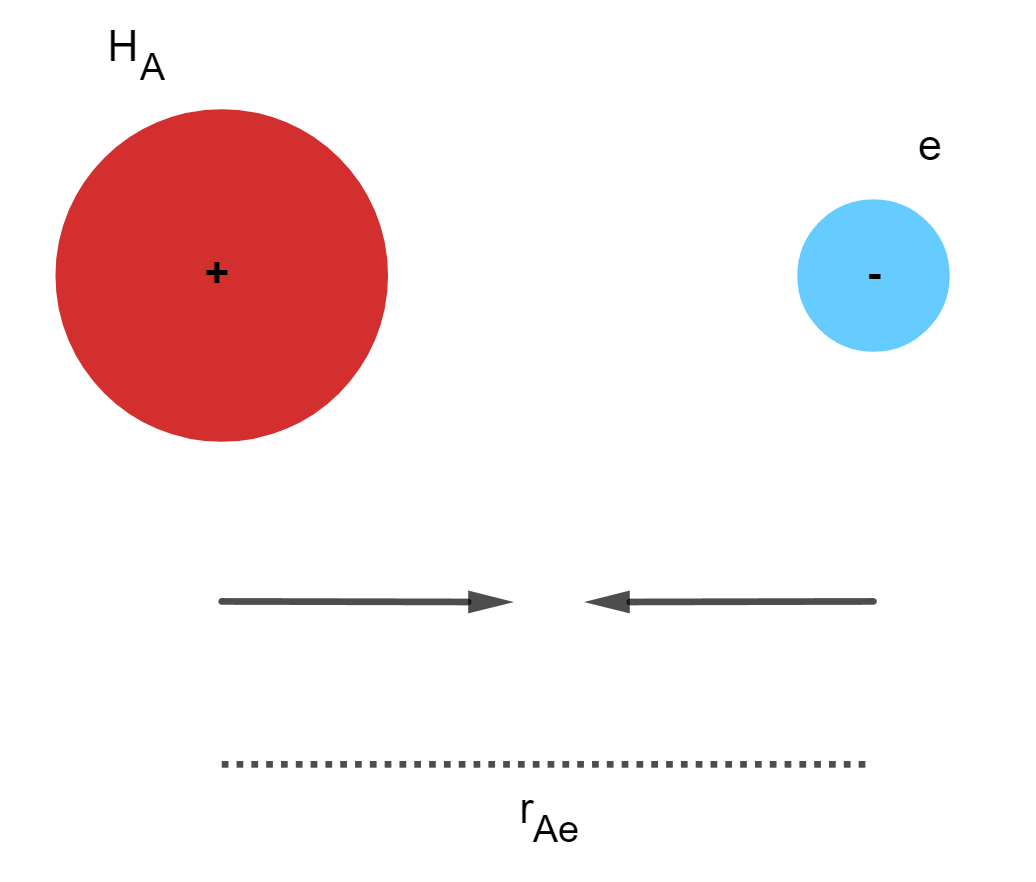
\includegraphics[width=4cm]{immagini/attrazione protone-elettrone.png}
    \end{figure}
    \end{minipage} \hfill
    \begin{minipage}{0.5\textwidth}
    \begin{figure}[H]
        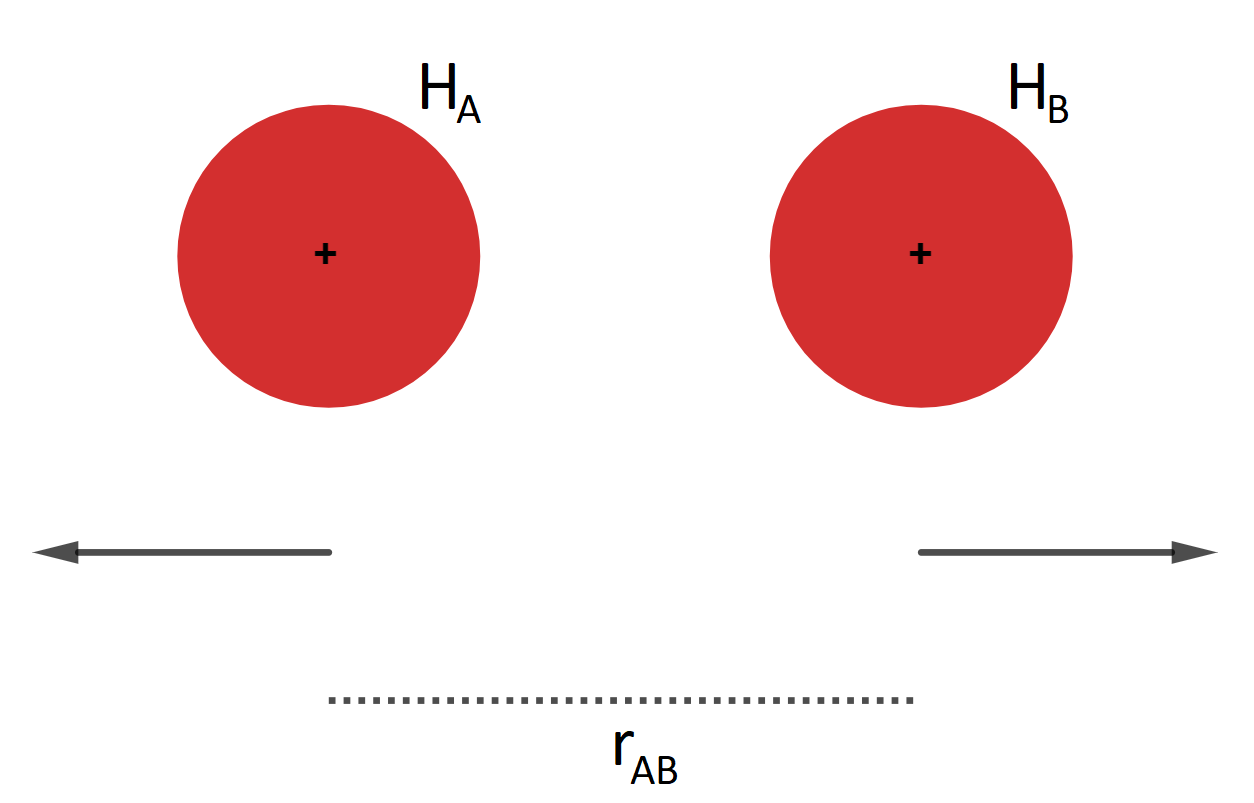
\includegraphics[width=5cm]{immagini/repulsione protone-protone.png}
    \end{figure}
    \end{minipage}

\comment{
    \begin{figure}[htp]
    \centering
    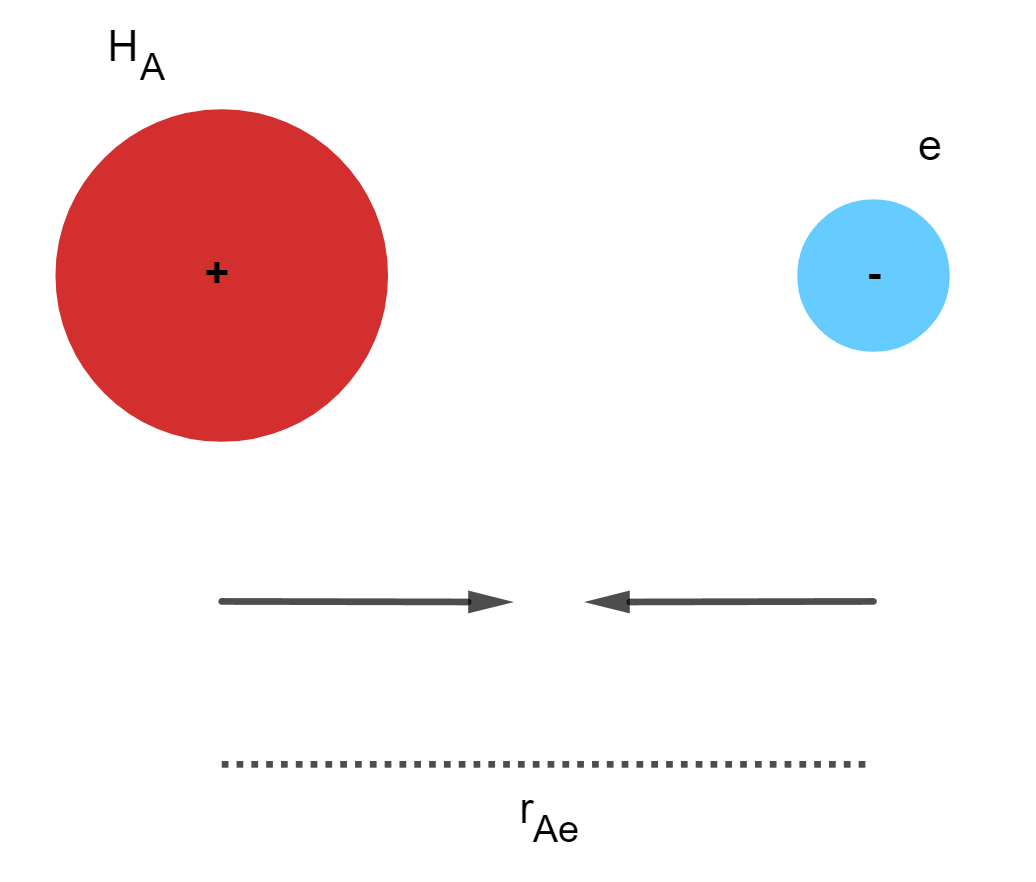
\includegraphics[width=4cm]{immagini/attrazione protone-elettrone.png}
\end{figure}
}
Una prima energia sarà data dall'attrazione tra l'elettrone con il nucleo dell'atomo di idrogeno A. Esso vale $E=\displaystyle-\frac{q^2}{r_{Ae}}$, ed essendo negativo abbassa l'energia del sistema.

Un secondo contributo analogo si avrà dall'attrazione tra elettrone e atomo di idrogeno B: $E=\displaystyle-\frac{q^2}{r_{Be}}$

\vspace{0.2cm}Un terzo e ultimo contributo sarà dato dalla repulsione tra i due nuclei. Tale energia vale $E=\displaystyle-\frac{q^2}{r_{AB}}$, ed essendo positivo alzerà l'energia.

\vspace{0.2cm}L'elettrone quindi interagisce con entrambi i nuclei:
\begin{figure}[htp]
    \centering
    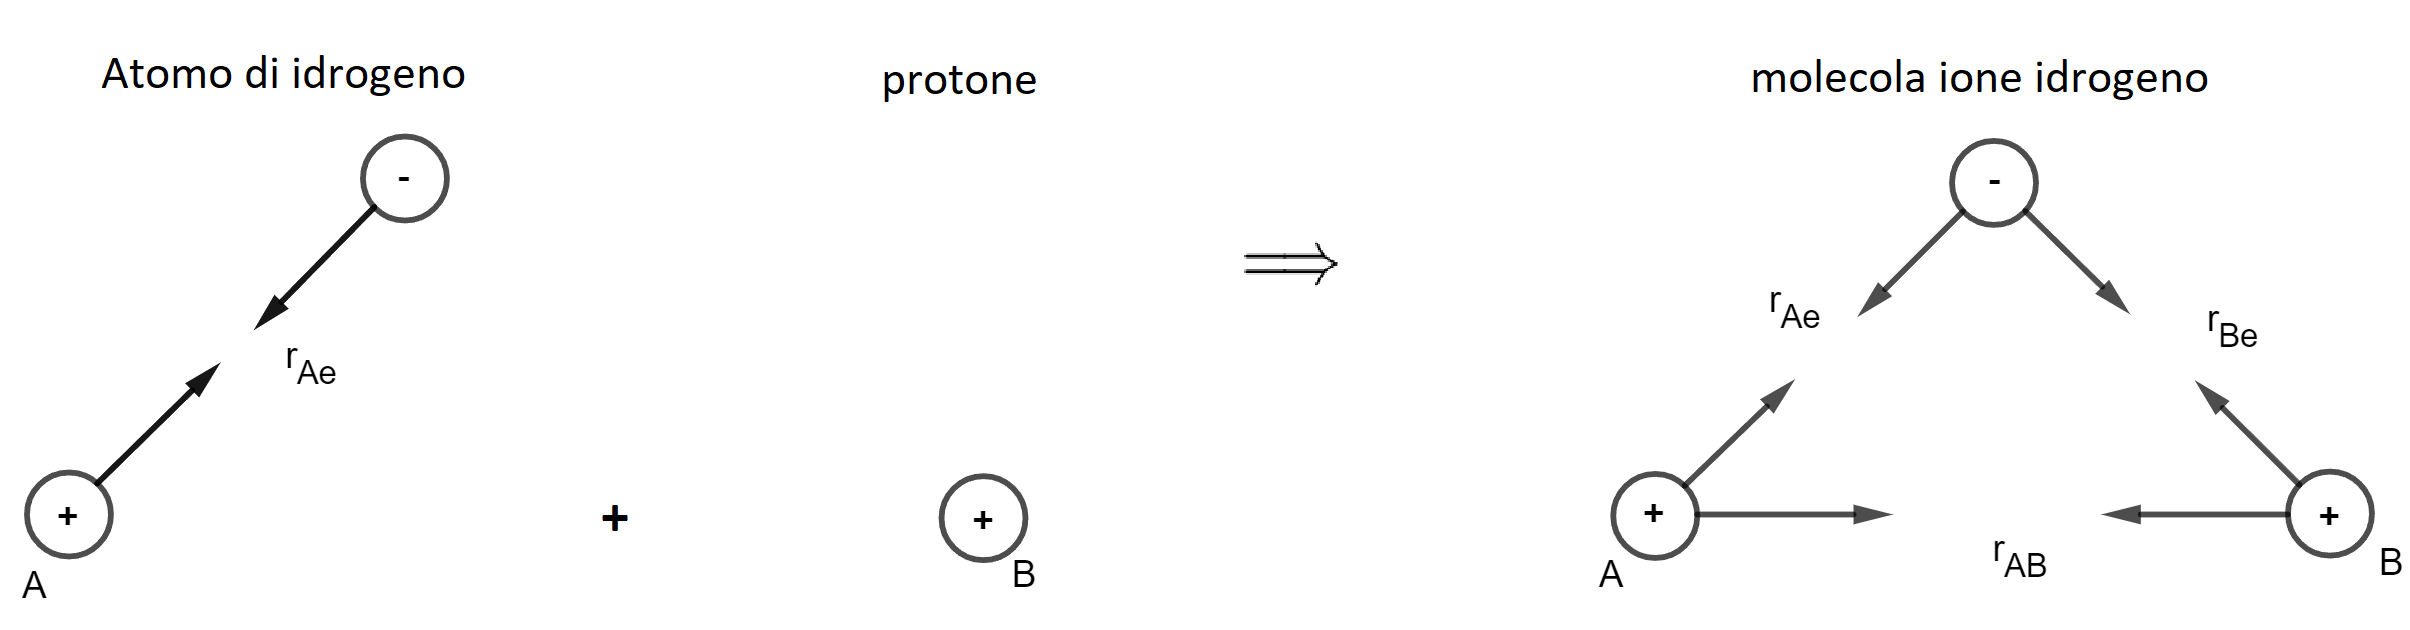
\includegraphics[width=14cm]{immagini/interazione_elettrone_con_protoni.png}
\end{figure}

Avremo tre distanze: quella tra il nucleo A e l'elettrone $r_Ae$, quella tra il nucleo B e l'elettrone $r_Be$ e quella tra i due nuclei $r_AB$.

Va da ricordare che la meccanica quantistica studia stati stazionari, cioè indipendenti dal tempo, il che significa che stiamo immaginando la molecola come se fosse rigida, cioè nel momento in cui andiamo a fare questi calcoli immaginiamo che non esistano vibrazioni ecc.

I termini energetici che avremo sono:
$$\ce{H_A^+-H_B^+ \quad + \quad H_A^+-e^- \quad + \quad H_B^+-e^-}$$
$$\text{repulsione \qquad attrazione \qquad attrazione}$$
$$\frac{q^2}{r_{AB}} \qquad - \qquad \frac{q^2}{r_{Ae}} \qquad - \qquad \frac{q^2}{r_{Be}}$$

Se immmaginiamo di avere particelle in posizioni fissate, possiamo andare a vedere qual è la composizione delle forze.

\begin{figure}[htp]
    \centering
    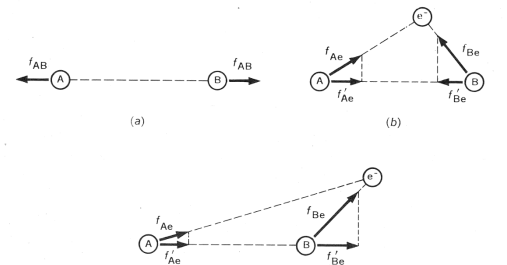
\includegraphics[width=10cm]{immagini/posizone_elettrone.png}
\end{figure}

Si nota che se questo elettrone, anziché essere fra i due nuclei fosse in una regione diversa (ad esempio a destra del nucleo B) sentirebbe l'attrazione di un nucleo, ma non è detto che senta quella dell'altro.

Quindi formalmente se l'elettrone viene immaginato come una particella, è chiaro che la sua posizione nello spazio è importante.

\vspace{0.2cm}Secondo la teoria degli orbitali molecolari, quando si formano molecole il numero di orbitali che ogni atomo possiede contribuirà agli orbitali molecolari che troveremo sulla molecola. Questo significa che se un atomo ha n orbitali di valenza, tutti questi contribuiranno a formare un ugual numero di orbitali molecolari.

In questo esempio abbiamo un orbitale $1s$ su ciascun atomo di idrogeno, per cui otterremo due orbitali molecolari: avremo una combinazione detta "\textit{in fase}" delle funzioni d'onda $1s_A + 1s_B$, e una combinazione detta  \textit{fuori fase} delle funzioni d'onda $1s_A - 1s_B$. La prima è detta \textit{combinazione di legame}, la seconda di \textit{antilegame}. In termini spaziali significa che per una data molecola lo spazio si divide in due regioni che daranno luogo, se è lì presente l'elettrone, alla combinazione legante e a quella antilegante:

\begin{figure}[htp]
    \centering
    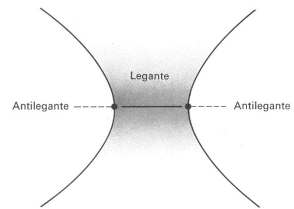
\includegraphics[width=6cm]{immagini/spazio_legante_antilegante.png}
\end{figure}

L'orbitale di antilegame si chiama così perché riempirlo non dà forza, anzi tende a distruggere il legame, a differenza di quello di legame che se riempito rafforza il legame.

Ne segue che di volta in volta dovremo fare i conti, in modo da capire quanti sono gli orbitali interagenti e quanti elettroni abbiamo a disposizione, in quanto le proprietà del legame dipenderanno da quanti orbitali di legame e quanti di antilegame si riempiranno.

\vspace{0.2cm}Sappiamo che sovrapporre due orbitali atomici di tipo $s$ significa ottenere orbitali molecolari di tipo $\sigma$. Supponiamo di avere due atomi di idrogeno distanti. Man mano che li avviciniamo, anche i loro orbitali atomici si avvicineranno, fino a sovrapporsi. Se ricordiamo l'andamento dell'energia potenziale, essa ha un minimo ad una distanza ben precisa sopra e sotto la quale l'energia è maggiore:

\begin{figure}[htp]
    \centering
    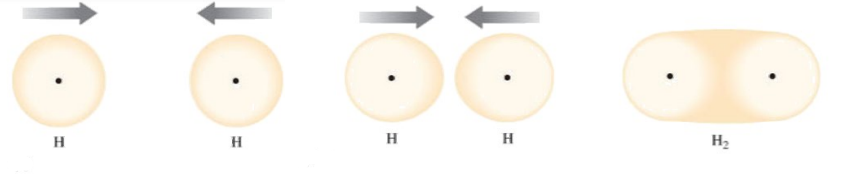
\includegraphics[width=12cm]{immagini/avvicinamento_orbitali.png}
\end{figure}

Supponiamo di essere alla distanza esatta che produce un minimo di energia. Essendoci un addensamento lungo la congiungente i nuclei ovvero lungo l'asse di legame, si ha un'interazione di tipo $\sigma$.

\vspace{0.2cm}Anche un orbitale $s$ con un orbitale $p$, e persino due orbitali $p$ orientati entrambi lungo l'asse di legame, danno luogo a un'interazione $\sigma$ che produce due orbitali: uno di legame  $\sigma$ e uno di antilegame  $\sigma^*$.

\hspace{0.2cm}\begin{minipage}{0.4\textwidth}
    \begin{figure}[H]
        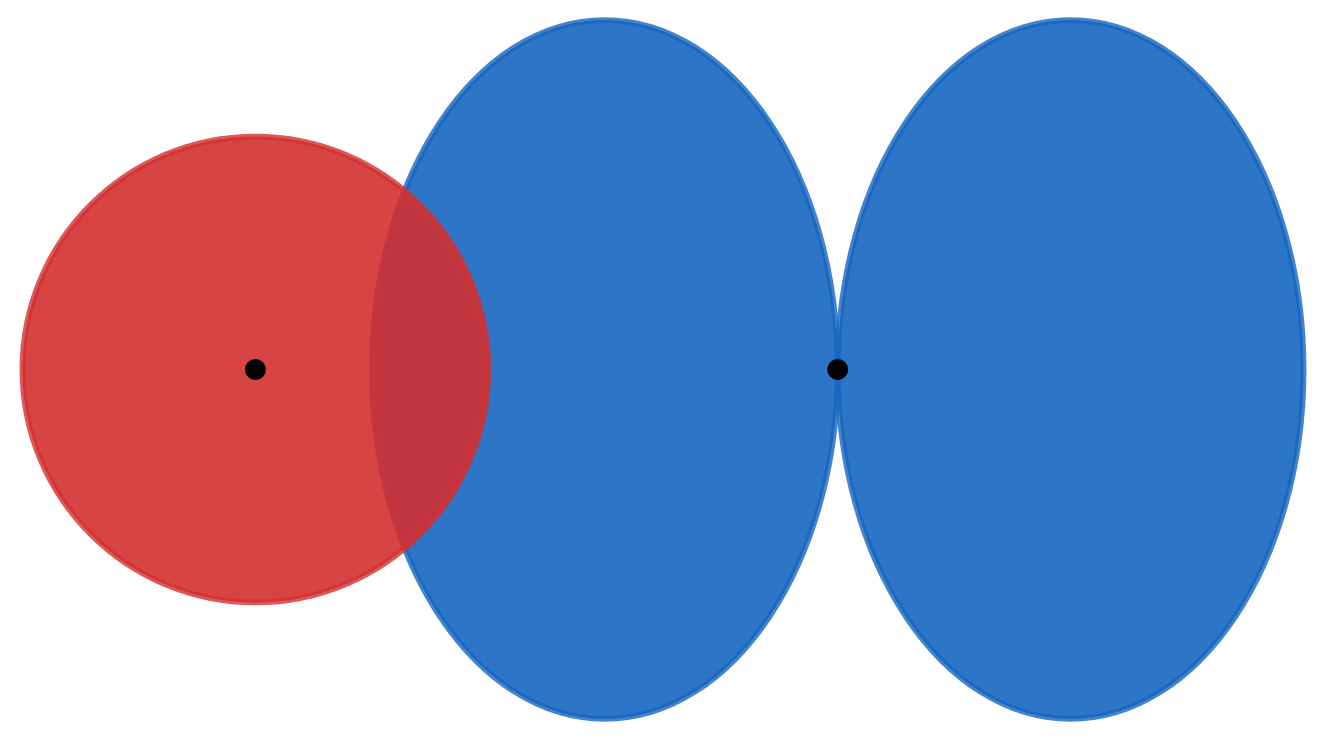
\includegraphics[width=5cm]{immagini/legame_sigma_s_p.png}
    \end{figure}
    \end{minipage} \hfill
\begin{minipage}{0.7\textwidth}
    \begin{figure}[H]
        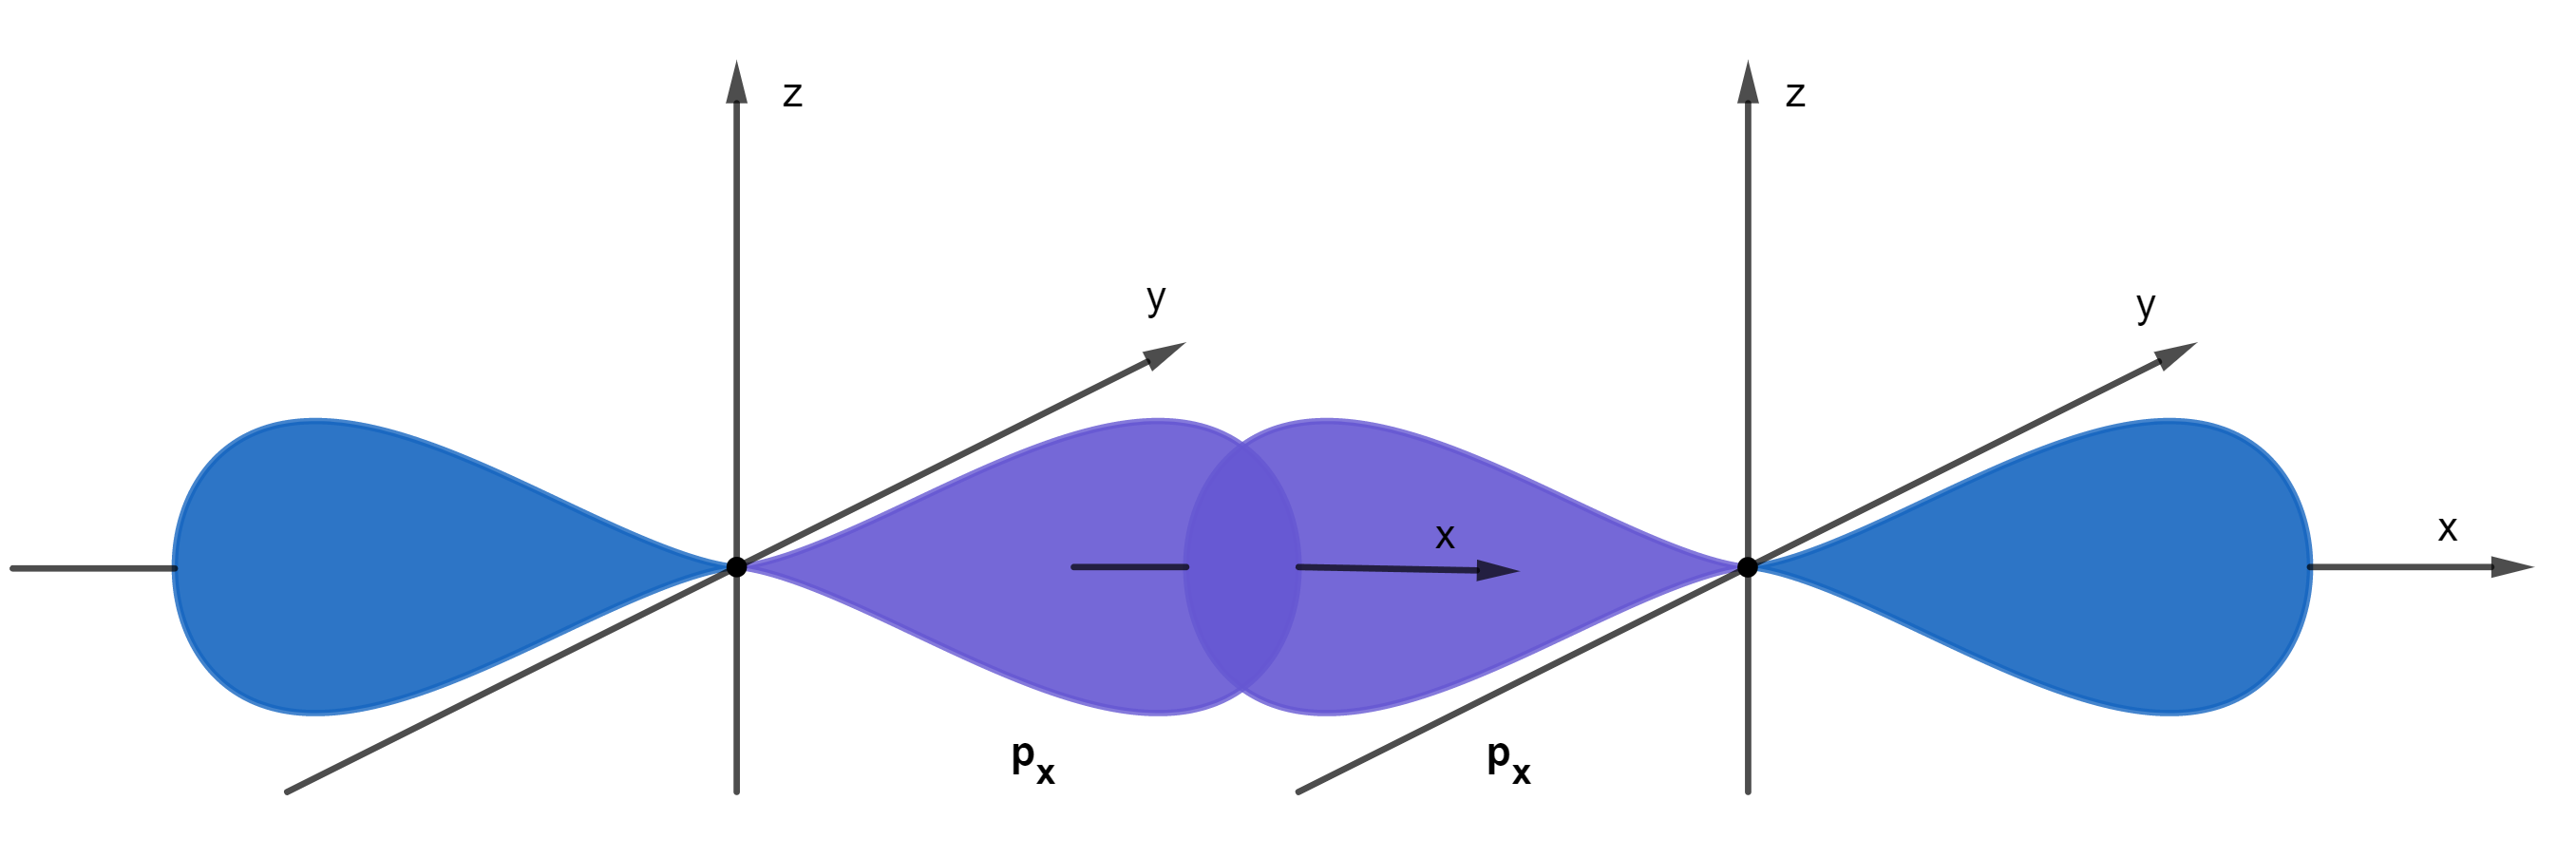
\includegraphics[width=9cm]{immagini/legame_sigma_p_p.png}
    \end{figure}
    \end{minipage}

(Nel grafico è riportata solo la combinazione di legame).
L'orbitale molecolare di legame sarà quello nel quale i lobi degli orbitali atomici interagenti (cioè le funzioni d'onda) hanno lo stesso segno, mentre in quello di antilegame hanno segno opposto.

Nel caso di interazione $\sigma$ tra due orbitali $p$, se abbiamo stabilito (come nel caso del grafico) che questi siano orientati lungo l'asse x, gli orbitali $p_y$ e $p_z$ saranno perpendicolari a tale asse e daranno lugo a sovrapposizioni $\pi$:

\hspace{1cm}\begin{minipage}{0.5\textwidth}
    \begin{figure}[H]
        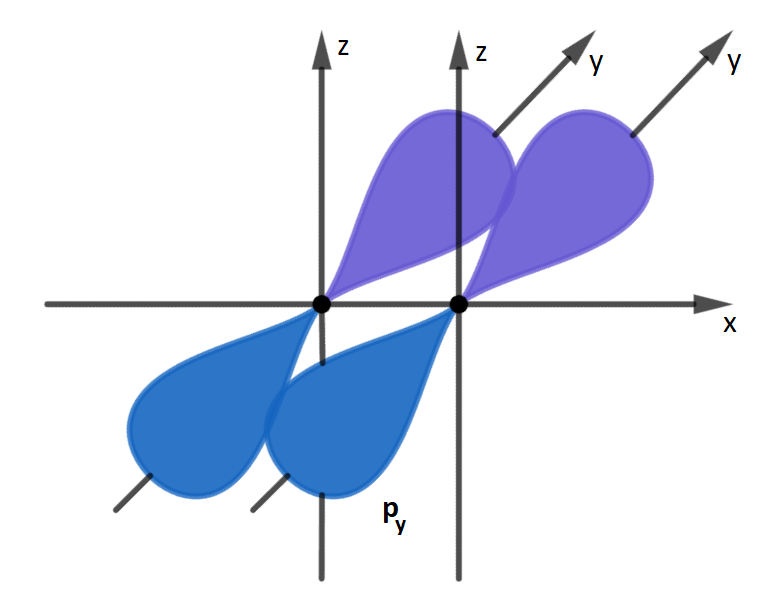
\includegraphics[width=7cm]{immagini/orbitali_py.png}
    \end{figure}
    \end{minipage} \hfill
    \begin{minipage}{0.5\textwidth}
    \begin{figure}[H]
        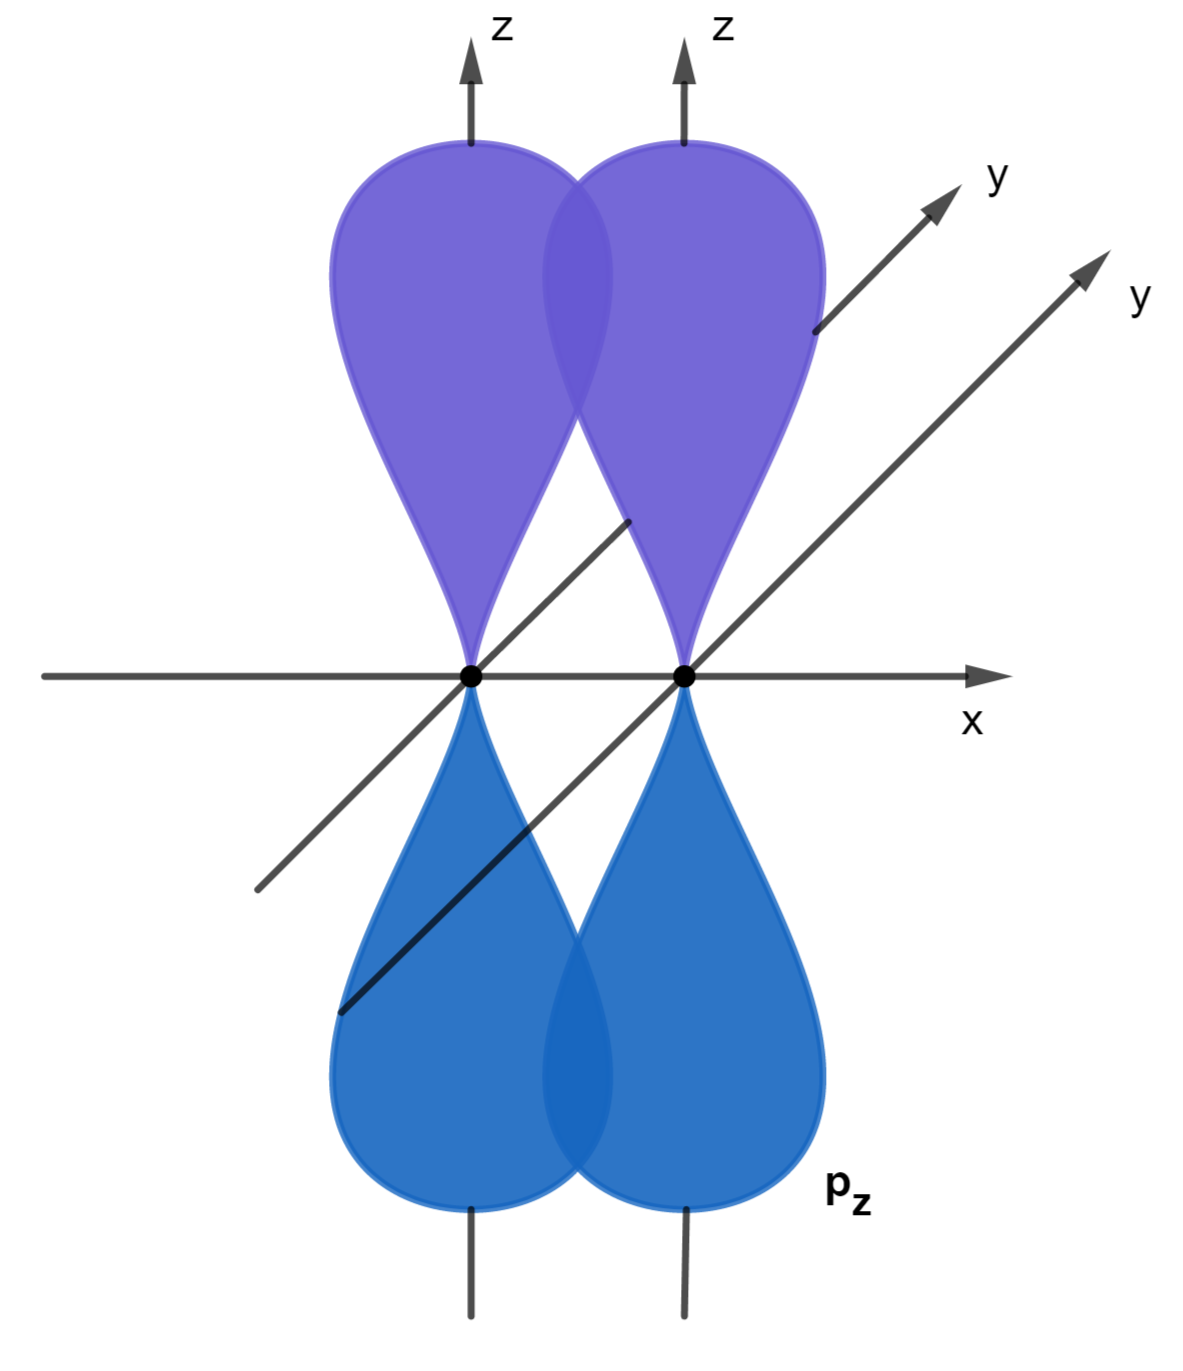
\includegraphics[width=5cm]{immagini/orbitali_pz.png}
    \end{figure}
    \end{minipage}


Quindi per una coppia di orbitali $p$ avremo una sovrapposizione diretta lungo la congiungente i due nuclei, mentre per le altre due coppie la sovrapposizione avverrà sopra e sotto.

\begin{minipage}{0.5\textwidth}
    \begin{figure}[H]
        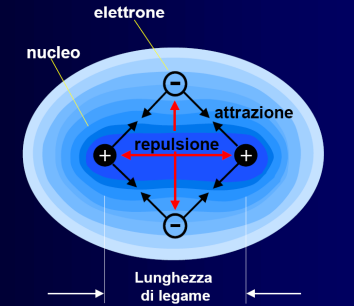
\includegraphics[width=7cm]{immagini/forze_legame_covalente.png}
    \end{figure}
    \end{minipage} \hfill
    \begin{minipage}{0.5\textwidth}
    \begin{figure}[H]
        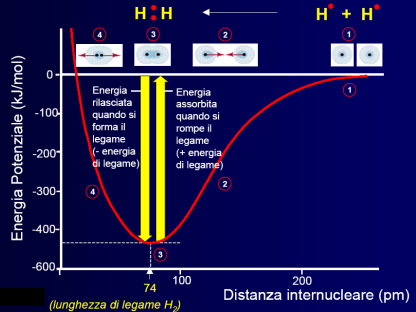
\includegraphics[width=8cm]{immagini/legame_covalente_H_2.png}
    \end{figure}
    \end{minipage}


\vspace{0.2cm}(In figura: Forze attrattive e repulsive nel legame covalente; Legame covalente nell'idrogeno H$_2$) 

\vspace{0.2cm}Questo è il modello che dobbiamo considerare quando studiamo composti nei quali il legame è covalente.

In questo caso non stiamo parlando di cessione di elettroni come invece se ne parla nel legame ionico.

Se abbiamo due nuclei di idrogeno e due elettroni, questi ultimi daranno luogo a forze attrattive in certe posizione rispetto ad altre.

Ruguardiamo la formazione della molecolaH$_2$: due atomi di idrogeno inizialmente molto distanti hanno energia potenziale praticamente nulla, ossia non interagiscono. Iniziamo ad avvicinare i due atomi e l'energia potenziale si abbassa. Appena le avviciniamo fino a 0.74 Å raggiungiamo il minimo. Si sono così formati i due orbitali molecolari, uno di legame e uno di antilegame. Se avviciniamo i due atomi ancora di più, l'energia potenziale tornerebbe a crescere a causa delle interazioni repulsive tra i nuclei e tra gli elettroni, i quali si troverebbero a occupare la stessa piccola regione di spazio. Quindi la distanza intermolecolare è importante al fine di capire se questo sistema ha raggiunto il minimo di energia.

Va da ricordare che per il sistema non sono possibili tutte le energie, ma solo alcuni valori quantizzati di questa.
\subsubsection{Orbitali molecolari leganti ed antileganti $\sigma$}

Ragioniamo ancora sulla molecola H$_2$.

Abbiamo due orbitali atomici, che chiameremo $1s(A)$ e $1s(B)$. Quando combiniamo le funzioni d'onda con lo stesso segno, avremo la combinazione \textit{in fase} o \textit{legante}, la cui funzione d'onda è data da una combinazione lineare delle funzioni d'onda atomiche:
$$\Psi(VB)=\Psi(1s)A + \Psi(1s)B \quad \text{(combinazione legante)}$$
Se invece i due orbitali $1s$ interagissero con funzioni d'onda il cui segno è opposto, avremo la combinazione \textit{fuori fase} o \textit{antilegante}:
$$\Psi^*(VB)=\Psi(1s)A - \Psi(1s)B \quad \text{(combinazione antilegante)}$$

Tracciamo una scala energetica:

\begin{figure}[htp]
    \centering
    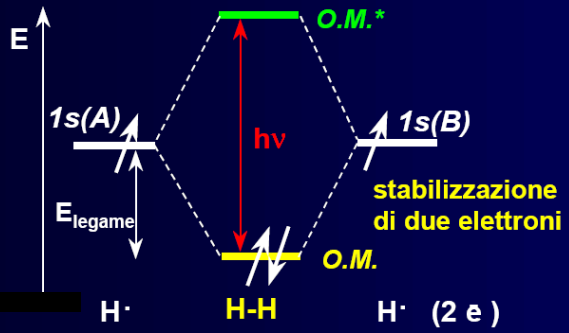
\includegraphics[width=7cm]{immagini/scala_energia_H_2.png}
\end{figure}

In questa scala qualitativa, abbiamo due orbitali di due atomi identici, quindi li mettiamo a pari livello. La freccia $\nearrow$ sta a indicare la presenza di un elettrone su ciascun orbitale.

Si avrà una interazione in fase con abbassamento di energia e una fuori fase con innalzamente in energia.

\begin{figure}[htp]
    \centering
    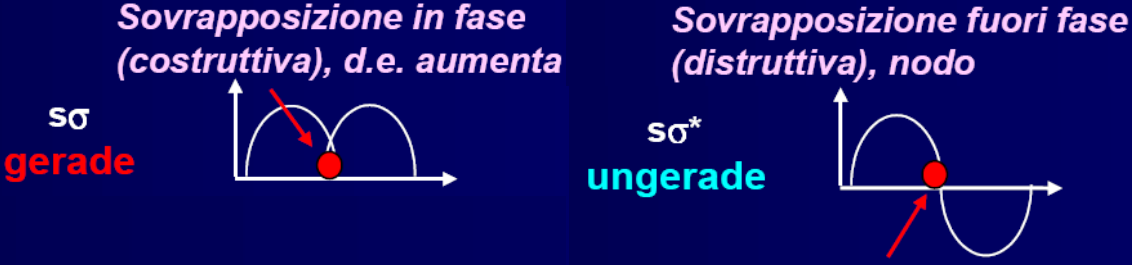
\includegraphics[width=12cm]{immagini/sovrapposizione_in_fase_e_fuori_fase.png}
\end{figure}

La funzione d'onda molecolare dell'orbitale legante mostra addensamento lungo la congiungente i nuclei, quella dell'ornitale legante mostra un nodo lungo essa.

\vspace{0.2cm}Dato che abbiamo solo due elettroni, entrambi andranno a riempire il livello più basso in energia. Quindi avremo una stabilizzazione netta di questi due elettroni, i quali prima si trovavano a un livello energetico più alto negli orbitali 1s, mentre adesso si trovano a energia più bassa perché la combinazione in fase si è stabilizzata.

Lasciamo invece vuoto l'orbitale molecolare di antilegame.
La molecola allora si forma perché c'è una stabilizzazione netta di questi due elettroni, che passano da una energia più alta ad una più basse.

Va da ricordare che quando si hanno queste interazioni verrà sepre mantenuto il baricentro di energia, ciò significa che la differenza di energia tra il livello di partenza e l'orbitale molecolare di legame sarà uguale alla differenza di energia tra il livello di partenza e l'orbitale molecolare di antilegame, ossia da un punto di vista energetico la destabilizzazione sarà uguale alla destabilizzazione, cioè le due quantità sono uguali.

La molecola H$_2$ quindi esiste solo perché nei fatti i due elettroni dei due atomi di idrogeno interagenti andranno a occupare il livello più basso in energia,avendo quindi un guadagno netto da un punto di vista energetico.

\subsubsection{L'ordine di legame (O.L.)}
Adesso possiamo esplicitare merglio il concetto di ordine di legame.

Esso va caclolato così:
$$\text{O.L.}=\frac{\text{n° di elettroni leganti - n° di elettroni antileganti}}{2}$$
dove gli elettroni leganti sono gli elettroni presenti negli orbitali di legame e quelli antileganti sono quelli presenti negli orbitali di antilegame.

Nel caso della molecola H$_2$ abbiamo 2 elettroni negli orbitali di legame e 0 elettroni in quelli di antilegame, per cui
$$\text{O.L.}=\frac{2-0}{2}=1$$

Essendo l'ordine di legame pari a 1, questa molecola si scrive con un legame semplice.

\vspace{0.2cm}Immaginiamo di avere due atomi di idrogeno A e B. La rappresentazione grafica delle loro funzioni d'onda è

\begin{figure}[htp]
    \centering
    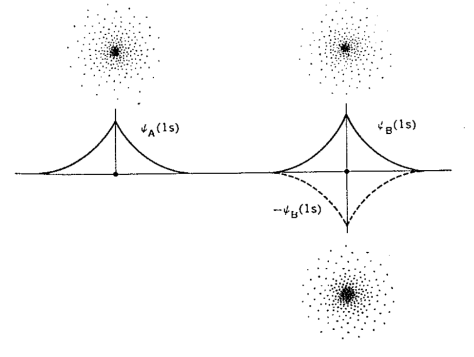
\includegraphics[width=10cm]{immagini/orbitali_atomici.png}
\end{figure}

Immaginiamo quindi di avvicinare i due nuclei, sia nel caso della combinazione in fase che in quello della combinazione fuori fase:

\begin{figure}[htp]
    \centering
    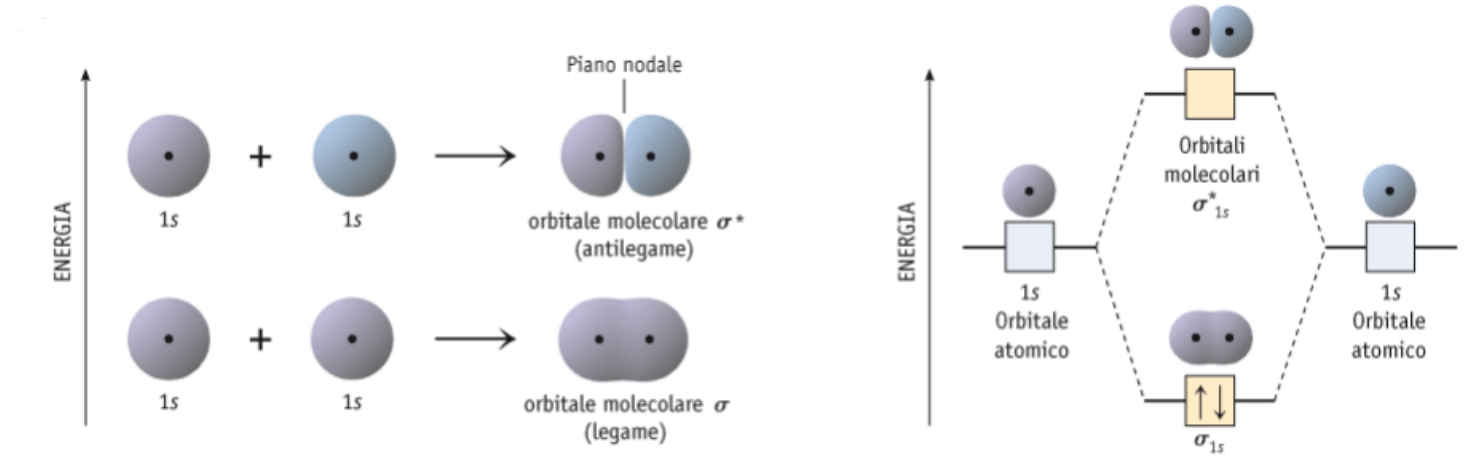
\includegraphics[width=14cm]{immagini/orbitali_molecolari_H_2.png}
\end{figure}

Se combiniamo due orbitali $1s$ con lo stesso segno di due atomi di idrogeno otterremo un orbitale molecolare di legame (di tipo $\sigma$ perché il legame avviene lungo la congiungente i nuclei).

Se combiniamo due orbitali $1s$ con segni diversi otteniamo un orbitale molecolare di antilegame, infatti abbiamo un nodo lungo l'asse di legame (di tipo $\sigma^*$).

\begin{figure}[htp]
    \centering
    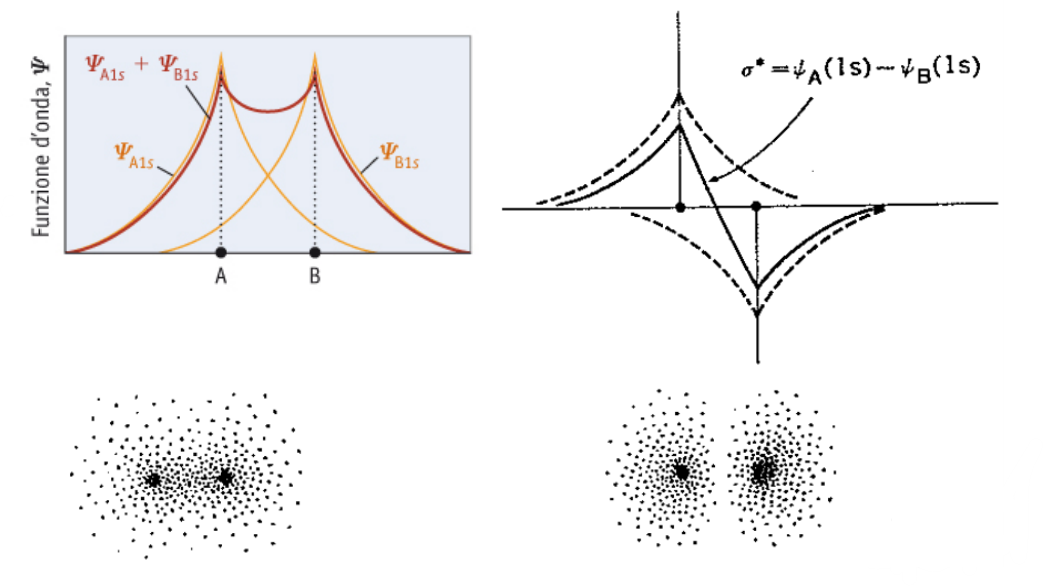
\includegraphics[width=12cm]{immagini/combinazione_funzioni.png}
\end{figure}

Possiamo quindi combinare sia due parti entrambe positive che una parte positiva e una negativa.

Nel primo caso quello che succede è che avvicinando i nuclei avremo una zona in comune, per cui la funzione si alza, cioè lungo la congiungente i nuclei, nell'orbitale $\sigma$ di legame, si avrà la funzione che cresce.

Al contrario, nell'altro caso, esattamente al centro tra i due nuclei la funzione si annulla (ci sarà un piano nodale).

Si ha quindi, ricapitolando, sovrapposizione di orbitali che rappresentiamo con la funzione d'onda. Aumenta l'ampiezza della funzione d'onda tra i due nuclei o viceversa diventa ero a seconda che si abbia combinazione in fase o fuori fase.

Dunque avremo sempre una combinazione in fase che darà luogo ad un orbitale $\sigma$ e una fuori fase che darà luogo a un orbitale $\sigma^*$. Dopodiché aggiungeremo gli elettroni, che nel caso della molecola H$_2$ occupano esclusivamente l'orbitale molecolare di legame.

Quindi sostanzialmente rispetto ad un valore di energia che possiamo immaginare essere il punto di riferimento (ossia l'energia degli orbitali non interagenti), avremo un abbassamento in energia della combinazione in fase e un innalzamento in energia della combinazione fuorifase.

\vspace{0.2cm}Iniziamo allora a vedere quanti elettroni riusciamo a sistemare in questo sistema costituito da due orbitali atomici interagenti che formano due orbitali molecolari:

\hspace{1.5cm}\begin{minipage}{0.1\textwidth}
    \begin{figure}[H]
        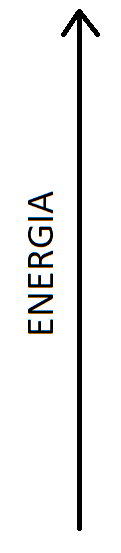
\includegraphics[width=1cm]{immagini/freccia_energia.png}
    \end{figure}
\end{minipage} \hfill
\begin{minipage}{0.95\textwidth}
        \begin{tabular}{m{4cm}|m{1.5cm}m{1.5cm}m{1.5cm}m{1.5cm}}
            \vspace{0.4cm}& \ce{H_2^+} & \ce{H_2} & \ce{He_2^+} & \ce{He_2}\\
            \vspace{0.4cm}$\boldsymbol{\sigma^*}(1s)$ & \vspace{0.4cm}\orbital{0} & \vspace{0.4cm}\orbital{0} & \vspace{0.4cm}\orbital{1} & \vspace{0.4cm}\orbital{2}\\
            \\
            \vspace{0.4cm}$\boldsymbol{\sigma}(1s)$ & \vspace{0.4cm}\orbital{1} & \vspace{0.4cm}\orbital{2} & \vspace{0.4cm}\orbital{2} & \vspace{0.4cm}\orbital{2}\\
            \vspace{0.4cm}Numero di elettroni & \vspace{0.4cm}\hspace{0.1cm}1 & \vspace{0.4cm}\hspace{0.1cm}2 & \vspace{0.4cm}\hspace{0.1cm}3 & \vspace{0.4cm}\hspace{0.1cm}4\\
            \vspace{0.2cm}Ordine di legame & \vspace{0.2cm}\hspace{0.05cm}$\displaystyle\frac{1}{2}$ & \vspace{0.2cm}\hspace{0.1cm}1 & \vspace{0.2cm}\hspace{0.05cm}$\displaystyle\frac{1}{2}$ & \vspace{0.2cm}\hspace{0.1cm}0
        \end{tabular}
\end{minipage}

\vspace{0.2cm}$\bullet$Esiste la molecola \ce{H_2^+}, avente due atomi di idrogeno e un solo elettrone, il quale andrà nell'orbitale più basso in energia. Rispetto all'energia del sistema di riferimento questa è più bassa, quindi questa molecola deve esistere. Il suo ordine di legame è 1/2;

\vspace{0.2cm}$\bullet$ Con la molecola H$_2$ riempiamo totalmente il livello più basso in energia con due elettroni. L'ordine di legame sarà 1, quindi per rappresentare questa molecola mettiamo un legame semplice.

\vspace{0.2cm}$\bullet$ L'elio è l'elemento successivo all'idrogeno, quindi ha due elettroni, ma l'orbitale continua a essere l'$1s$, per cui nella molecola He$_2$ si genera ancora un orbitale $\sigma$ e uno $\sigma^*$. Stavolta però avremo in totale quattro elettroni, il che significa che riempiamo totalmente sia l'orbitale di legame che quello di antilegame. Da ciò capiamo che non ci sarà alcun guadagno in energia rispetto alla situazione dei due atomi non interagenti, perché avendo mantenuto il baricentro di energia l'energia guadagnata riempiendo totalmente l'orbitale di legame è uguale a quella persa riempiendo l'orbitale di antilegame.

L'ordine di legame allora sarà pari a zero. il che significa che questa molecola non puà esistere, e nei fatti l'elio non esiste in forma molecolare.

\vspace{0.2cm}$\bullet$ Supponiamo per assurdo che l'He$_2$ esista e strappiamogli un elettrone: otterremo la specie He$_2^+$, avente tre elettroni. Due di questi riempiranno l'orbitale molecolare di legame e solo uno riempirà parzialmente quello di antilegame. Siccome due elettroni si stabilizzano e solo uno si destabilizza, si avrà un guadagno in energia. Infatti anche l'ordine di legame risulta diverso da zero: esso è pari a 1/2.

In questo modo dimostriamo che non può esistere la molecola He$_2$, ma esiste il suo catione He$_2^+$.

\vspace{0.2cm} Ciò che stiamo studiando è l'esito di una trattazione quanto-meccanica, e per questi sistemi il modello che ci propone la meccanica quantistica è perfetto perché nei fatti ci permette di razionalizzare l'esistenza o meno di alcune molecole.

\vspace{0.2cm}Consideriamo adesso il litio, che è un metallo.

Immaginiamo la molecola fatta da due atomi di litio. Può esistere questa molecola?

Consideriamo gli orbitali coinvolti, i quali non sono tutti, perché se abbiamo l'orbitale $2s$ dobbiamo avere anche gli orbitali $2p$, in quanto avendo il numero quantico principale pari a 2, l può valere 0 (orbitali s) o 1 (orbitali p). Tuttavia non abbiamo elettroni a sufficienza per riempire i livelli $2p$, quindi non li rappresenteremo:

\begin{minipage}{0.5\textwidth}
    \begin{figure}[H]
    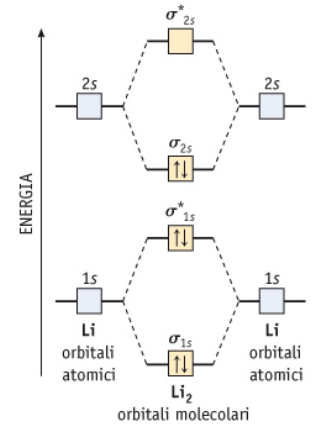
\includegraphics[width=7cm]{immagini/orbitali_molecolari_Li_2.png}
    \end{figure}
    \end{minipage} \hfill
    \begin{minipage}{0.5\textwidth}
        \vspace{0.5cm}Abbiamo gli orbitali $1s$ totalmente pieni perché nel litio l'$1s$ è pieno con due elettroni, quindi in totale ne avremo quattro. Avremo poi la combinazione in fase e quella fuorifase dei due livelli $1s$. Dunque abbiamo due orbitali molecolari con quattro elettroni, quindi riempiamo totalmente sia l'orbitale $\sigma$ che quello $\sigma^*$, pertanto questi elettroni non contribuiranno all'ordine di legame (2-2=0), ossia questi livelli non contribuiscono al legame chimico nella molecola Li$_2$.

        \vspace{0.2cm}Andiamo adesso all'orbitale $2s$. Va da ricordare che il litio sta sotto l'idrogeno, per cui la sua configurazione elettronica esterna è $2s^1$, cioè un solo elettrone.
        
        Quello che vale per gli $1s$ vale anche per i $2s$, quindi avremo un'altra combinazione in fase $\sigma_{2s}$ e una fuorifase $\sigma_{2s}^*$. Abbiamo solo due elettroni in totale, i quali andranno ad occupare il livello più basso in energia, cioè l'orbitale $\sigma_{2s}$, lasciando vuoto il $\sigma_{2s}^*$. Già da ciò capiamo che questa molecola ha una sua stabilità.
        
        Se andiamo a calcolare l'ordine di legame avremo (4-2)/2=1: la molecola Li$_2$ esiste e va scritta con un legame semplice \ce{Li-Li}.
    \end{minipage}

\vspace{0.4cm}Va da notare che non era nemmeno necessario rappresentare i livelli $1s$ perché sono a numero quantico inferiore, per cui non sono di valenza.

\vspace{0.2cm}Andiamo a ragionare sugli orbitali p:

\begin{figure}[htp]
    \centering
    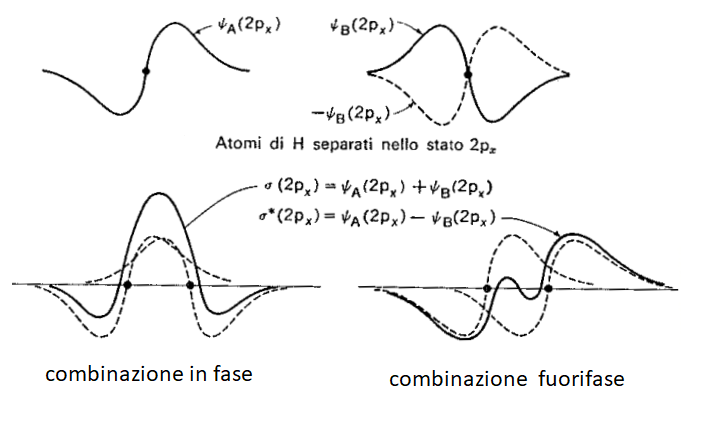
\includegraphics[width=10cm]{immagini/orbitali_molecolari_pigreco.png}
\end{figure}

Con "atomi di idrogeno separati nello stato $2p_z$" si intende che gli orbitali sono stati ottenuti come soluzioni esatte dell'equazione di Schrödinger scritta per l'atomo di idrogenom ma poi le usiamo per qualunque altro atomo. Quindi non dobbiamo scordare che quando rappresentiamo gli orbitali stiamo usando gli orbitali ottenuti per l'atomo di idrogeno, perché quelli rappresentano le soluzioni esatte. Stiamo anche pensando che sia ragionevole usare questi orbitali anche per atomi polielettronici, tenuto conto del fatto che ciò che cambia sarò la diversa penetrazione rispetto al nucleo, visto che ci saranno orbitali interni pieni e pertanto schermanti rispetto agli elettroni esterni, e la diversa carica nucleare efficace sentita dagli elettroni esterni dunque. Ne abbiamo parlato studiando la teoria atomica: noi apportiamo delle correzioni a questi sistemi, ma quando rappresentiamo le forme degli orbitali usiamo sempre gli orbitali dell'atomo di idrogeno. Quindi indipendentemente dal fatto che l'atomo di idrogeno, nel suo stato fondamentale, possiede un elettrone solo nell'orbitale $1s$, per quest'atomo possiamo ottenere tutte le funzioni ($1s, \; 2s, \; 2p, \; 3s, \; 3p, \; 3d, \; 4s, \; 4p, \; 4d, \; 4f$ e anche oltre).

\vspace{0.2cm}Se avviciniamo i due nuclei, avremo una sovrapposizione delle funzioni d'onda per quanto attiene alla combinazione lineare. Si ha un addensamento, cioè aumenta l'ampiezza della funzione d'onda lungo la congiungente i nuclei.

Se invece facciamo interagire una funzione d'onda con l'altra negativa otteniamo un nodo al centro, lungo l'asse di legame, che non esiste nella composizione in fase.

\begin{figure}[htp]
    \centering
    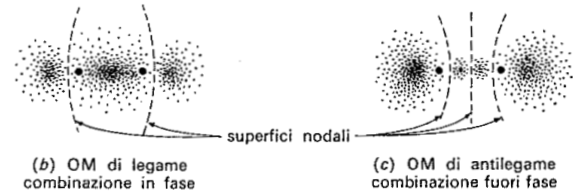
\includegraphics[width=8cm]{immagini/orbitali_molecolari_pigreco_nuvoletta.png}
\end{figure}

Usiamo la rappresentazione a nuvolette. In essa abbiamo un addensamento dei puntini della nuvoletta lungo l'asse di legame per la combinazione in fase, al contrario avremo un nodo nella combinazione fuori fase. Va poi da ricordare che la funzione $p$ di per sé ha un nodo: essa cambia segno all'origine degli assi. Ne segue che nella combinazione in fase avremo tre lobi più i due nodi all'origine mentre nella combinazione fuori fase avremo quattro lobi e tre nodi.

Graficamente:

\begin{figure}[htp]
    \centering
    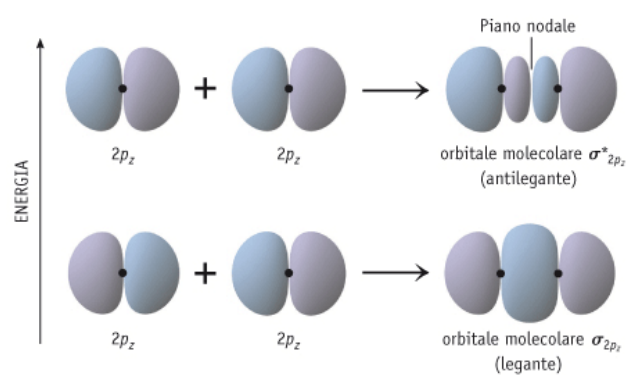
\includegraphics[width=8cm]{immagini/orbitali_sigma_p.png}
\end{figure}

Questo vale per gli orbitali che puntano lungo l'asse di legame, i quali daranno luogo a combinazione $\sigma$ di legame e di antilegame.

Consideriamo gli orbitali $p$ perpendicolari a quest'asse:

\begin{figure}[htp]
    \centering
    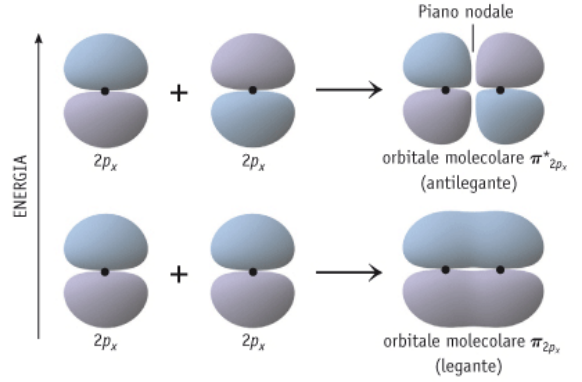
\includegraphics[width=8cm]{immagini/orbitale_pigreco_p.png}
\end{figure}
Tali orbitali daranno luogo ad una combinazione in fase, ma perpendicolarmente all'asse di legame, ossia stavolta lungo l'asse di legame ci sarà un piano nodale; e ad una combinazione fuori fase.

Gli orbitali perpendicolari all'asse di legame in totale sono quattro, quindi daranno luogo a 4 orbitali molecolari, due in fase e due fuori fase.

Non contando gli orbitali $s$, abbiamo tre orbitali $p$ su ogni atomo ($p_x, \; p_y, \; p_z$) e in totale ne avremo sei, da cui segue che avremo sei orbitali molecolari: tre in fase e tre fuori fase.
In termini di energia si ha:

\begin{figure}[htp]
    \centering
    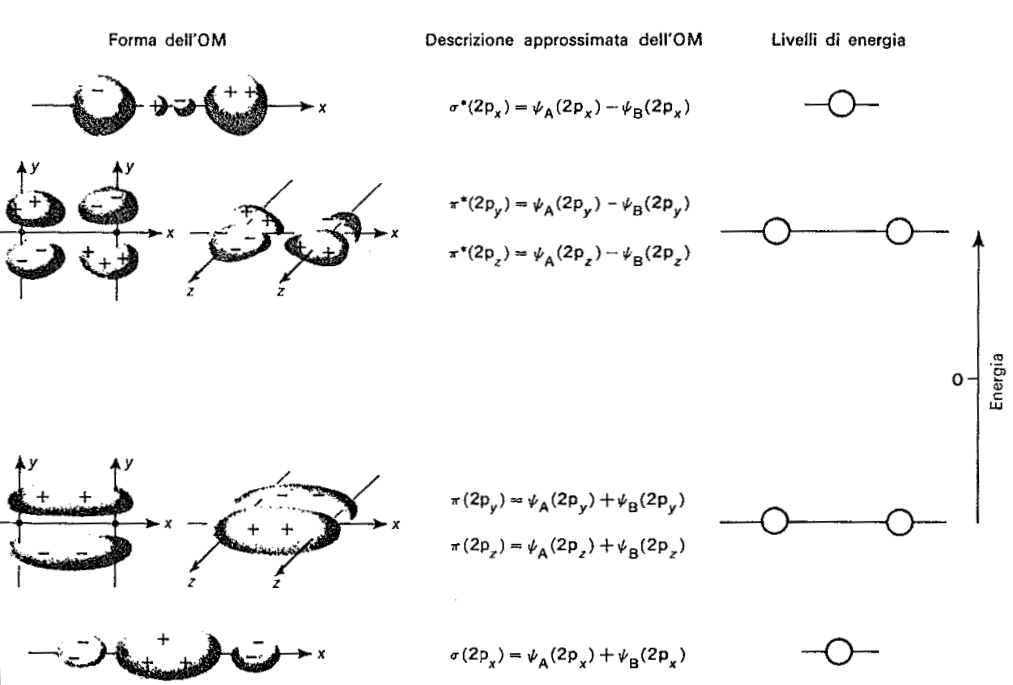
\includegraphics[width=8cm]{immagini/equazioni_orbitali.png}
\end{figure}

Due orbitali $p_x$ che putano l'uno sull'altro danno luogo alla configurazione $\sigma_p$ di legame e $\sigma^*_p$ di antilegame, le quali da un punto di vista energetico stanno rispettivamente più in basso e più in alto.

I due set $p_y$ e $p_z$ perpendicolari all'asse di legame danno luogo alle combinazioni $\pi$ di legame e $\pi^*$ di antilegame.

Gli orbitali $\pi_{2p_y}$ e $\pi_{2p_z}$, così come avviene per i $\pi_{2p_y}^*$ e $\pi_{2p_z}^*$, sono degeneri, ossia sono allo stesso livello di energia.

In totale riempiremo gli orbitali, sia di legame che di antilegame, con 12 elettroni. Con 12 elettroni la molecola si distrugge, fino a 11 siamo a posto.

La sequenza, dall'energia più bassa a quella più alta, degli orbitali molecolari generati a partire da orbitali $p$ è: $\sigma, \; \pi, \; \pi^*, \; \sigma^*$.

Si ha però un'anomalia: boro, carbonio e azoto hanno una differenza energetica tra gli orbitali $2s$ e gli orbitali $2p$ più piccola di quella osservata subito dopo, cioè dall'ossigeno in poi. Ragionando in kcal/mol, la differenza energetica tra gli orbitali $2s$ e i $2p$ di B, C, N è di circa 100 kcal/mol. Tal edifferenza arriva a 300 quando si arriva all'ossigeno.

\begin{figure}[htp]
    \centering
    \includegraphics[width=6cm]{immagini/differenza_energia_2s_2p.png}
\end{figure}

Il motivo è che prima dei livelli $2p$ abbiamo i livelli $2s$, e se la distanza energetica tra questi livelli è piccola ciò che succede è che i livelli $\sigma_{2s}$ e $\sigma_{2s}^*$ si abbassano in energia e l'orbitale $\sigma_{2p}$ che è subito dopo si alza in energia a tal punto da capovolgere l'ordine, ossia quest'orbitale, interagendo con quelli più interni, si sposta fino a superare l'energia dei livelli $\pi_{2p}$. Quindi per boro, carbonio e azoto la sequenza energetica è $\pi,\; \sigma, \; \pi^*, \; \sigma^*$

\begin{figure}[htp]
    \centering
    \includegraphics[width=10cm]{immagini/livelli_B2_C2_N2.png}
\end{figure}

Vediamo in dettaglio tutte le forme degli orbitali:

\begin{figure}[htp]
    \centering
    \includegraphics[width=10cm]{immagini/sequenza_energetica_BCN.png}
\end{figure}

\begin{itemize}
    \item Partendo dagli $1s$, la combinazione di due di questi orbitali darà luogo ad un $\sigma$ ed un $\sigma^*$;
    \item Anche i livelli $2s$ danno luogo ad un $\sigma$ ed un $\sigma^*$;
    \item I tre orbitali atomici $p$ presenti su ciascun atomo daranno luogo alle combinazioni, in ordine energetico crescente, $\pi,\; \sigma, \; \pi^*, \; \sigma^*$. A questo punto sarà solo una questione di riempimento.
\end{itemize}

Consideriamo la molecola N$_2$. Col formalismo di Lewis la rappresentavamo con un legame triplo. Contando anche i livelli $1s$, ogni azoto ha 7 elettroni per un totale di 14. Se andiamo a riempire gli orbitali molecolari, arriveremo al $\sigma_{2p}$. Gli elettroni di legame sono 10, quelli di antilegame 4. L'ordine di legame è pari a (10-4)/2=3, ed ecco perché si usa un triplo legame per rappresentare tale molecola. Quindicon la teoria degli orbitali molecolari arriviamo alla stessa risposta ottenuta con l'approccio di Lewis.

\vspace{0.2cm}
Dall'ossigeno in poi ritorniamo al diagramma inizialmente discusso, ossia la sequenza energetica è $\sigma_{1s}, \; \sigma^*_{1s}, \; \sigma_{2s}, \; \sigma^*_{2s}, \; \sigma_{2p}, \; \pi_{2p}, \; \pi^*_{2p}, \; \sigma^*_{2p}$.

Vediamo che cosa succede alla molecola di ossigeno con questa trattazione.

Ogni ossigeno fornisce, contando anche i liveli $1s$, 8 elettroni, per cui dovremo posizionare 16 elettroni. Con 14 elettroni arriviamo a riempire fine ai livelli $\pi$. I due elettroni restanti, dato che gli orbitali $\pi^*$ sono degeneri, possono stare entrambi nello stesso orbitale oppure stanno uno su un orbitale e uno sull'altro. Queste due situazioni sono a energie diverse, in quanto se possibile gli elettroni preferiscono stare con spin paralleli in orbitali diversi. Accoppiare lo spin di due elettroni significa sempre spendere energia, quindi quando stanno nello stesso orbitale siamo a energia maggiore. Pertanto la situazione a energia più bassa si ha quando gli elettroni hanno spin paralleli ma stanno in orbitali diversi. Inoltre la situazione a più alta energia non è lo stato fondamentale dell'ossigeno.

Ragioniamo ora in termini di molteplicità di spin, pari a $2S + 1$, dove $S$ è lo spin totale (che è un numero relativo agli atomi). Questi due stati vengono chiamati \textbf{stato di tripletto} e \textbf{di singoletto}, in quanto nel caso in cui gli elettroni stiano in orbitali diversi, entrambi avranno spin pari a 1/2, per cui $2(1/2 + 1/2)+1=2 \cdot 1 + 1=3$, mentre nel caso in cui essi sono costretti nello stesso orbitale avranno spin opposti, cioè uno pari a 1/2 e l'altro pari a -1/2 e quindi si ha $2(1/2 - 1/2) + 1= 2 \cdot 0 + 1=1$.
\begin{center}
\begin{tabular}{m{4.2cm}m{4cm}m{4cm}}
    \hspace{0.4cm}$\sigma^*_{2px}$ & \hspace{0.4cm}\vspace{-0.2cm}\orbital{0} & \hspace{0.4cm}\vspace{-0.2cm}\orbital{0}\\
    \vspace{0.4cm}$\pi^*_{2py} \quad \pi^*_{2pz}$ & \hspace{0.15cm}\vspace{-0.5cm}\orbitals{20} & \hspace{0.15cm}\vspace{-0.5cm}\orbitals{11}\\
    \vspace{0.4cm}$\pi_{2py} \quad \pi_{2pz}$ & \hspace{0.15cm}\vspace{-0.5cm}\orbitals{22} & \hspace{0.15cm}\vspace{-0.5cm}\orbitals{22}\\
    \vspace{0.4cm}\hspace{0.4cm}$\sigma_{2px}$ & \hspace{0.4cm}\vspace{-0.5cm}\orbital{2} & \hspace{0.4cm}\vspace{-0.5cm}\orbital{2}\\
    \vspace{0.4cm}\hspace{0.4cm}$\sigma^*_{2s}$ & \hspace{0.4cm}\vspace{-0.5cm}\orbital{2} & \hspace{0.4cm}\vspace{-0.5cm}\orbital{2}\\
    \vspace{0.4cm}\hspace{0.4cm}$\sigma_{2s}$ & \hspace{0.4cm}\vspace{-0.5cm}\orbital{2} & \hspace{0.4cm}\vspace{-0.5cm}\orbital{2}\\
    \vspace{0.4cm}\hspace{0.4cm}$\sigma^*_{1s}$ & \hspace{0.4cm}\vspace{-0.5cm}\orbital{2} & \hspace{0.4cm}\vspace{-0.5cm}\orbital{2}\\
    \vspace{0.4cm}\hspace{0.4cm}$\sigma_{1s}$ & \hspace{0.4cm}\vspace{-0.5cm}\orbital{2} & \hspace{0.4cm}\vspace{-0.5cm}\orbital{2}\\
    \vspace{0.4cm}Nome & \vspace{0.4cm}singoletto & \vspace{0.4cm}tripletto\\
    \vspace{0.3cm}Energia & \vspace{0.3cm}+22.5 kcal/mol & \vspace{0.3cm}0\\
    \vspace{0.3cm}Energia di legame & \vspace{0.3cm}96 kcal/mol & \vspace{0.3cm}118 kcal/mol\\
    \vspace{0.3cm}Lunghezza di legame & \vspace{0.3cm}1.22 Å & \vspace{0.3cm}1.21 Å\\
    \vspace{0.3cm}Costante di forza & \vspace{0.3cm}10.7 mdine/Å & \vspace{0.3cm}11.4 mdine/Å\\
    \vspace{0.3cm}Ordine di legame apparente & \vspace{0.3cm}2 & \vspace{0.3cm}2\\
    \vspace{0.3cm}Proprietà magnetiche & \vspace{0.3cm}non magnetico & \vspace{0.3cm}magnetico
\end{tabular}
\end{center}
Se scegliamo lo stato di tripletto come zero di energia, per ottenere lo stato di singoletto dobbiamo spendere 22.5 kcal/mol, infatti è un sistema a più alta energia cioè è meno stabile, tant'è vero che l'energia di legame è minore, la lunghezza di legame è maggiore e, immaginando il legame chimico come una molla, possiamo definire una costante di forza, che risulta minore nel singoletto. L'ordine di legame invece non cambia, perché sia quando stanno sullo stesso orbitale che quando stanno su orbitali diversi si trovano comunque in orbitali di antilegame. In particolare per entrambi gli stati risulta un ordine di legame pari a 2, quindi rappresentiamo l'O$_2$ con un doppio legame. 

Inoltre si ha che se gli elettroni sono appaiati (stato di singoletto) l'ossigeno sarà diamagnetico, se sono spaiati (stato di tripletto) il sistema sarà paramagnetico. Ciò è vero: l'ossigeno liquido viene trattenuto tra le espansioni di un magnete.

\vspace{0.2cm}Graficamente, la disposizione degli elettroni negli orbitali (non considerando quelli a numero quantico inferiore) è la seguente:
\begin{center}
\begin{tabular}{ m{3.2cm}m{1cm}m{1cm}m{1cm}|m{1cm}m{1cm}m{1cm}m{1cm}}
    & $\mathbf{B_2}$ & $\mathbf{C_2}$ & $\mathbf{N_2}$ & & $\mathbf{O_2}$ & $\mathbf{F_2}$ & $\mathbf{He_2}$\\
    \vspace{0.4cm}$\boldsymbol{\sigma^*}_{2p}$ & \vspace{0.2cm}\orbital{0} & \vspace{0.2cm}\orbital{0} & \vspace{0.2cm}\orbital{0} & \vspace{0.4cm}$\boldsymbol{\sigma^*}_{2p}$ & \vspace{0.2cm}\orbital{0} & \vspace{0.2cm}\orbital{0} & \vspace{0.2cm}\orbital{2}\\
    \vspace{0.4cm}$\boldsymbol{\pi^*}_{2p}$ & \hspace{-0.25cm}\vspace{-0.4cm}\orbitals{00} & \hspace{-0.25cm}\vspace{-0.4cm}\orbitals{00} & \hspace{-0.25cm}\vspace{-0.4cm}\orbitals{00} & \vspace{0.4cm}$\boldsymbol{\pi^*}_{2p}$ & \hspace{-0.25cm}\vspace{-0.4cm}\orbitals{11} & \hspace{-0.25cm}\vspace{-0.4cm}\orbitals{22} &\hspace{-0.25cm}\vspace{-0.4cm}\orbitals{22}\\
    \vspace{0.4cm}$\boldsymbol{\sigma}_{2p}$ & \vspace{0.4cm}\orbital{0} & \vspace{0.4cm}\orbital{0} & \vspace{0.4cm}\orbital{2} & \vspace{0.4cm}$\boldsymbol{\pi}_{2p}$ & \hspace{-0.25cm}\vspace{-0.4cm}\orbitals{22} & \hspace{-0.25cm}\vspace{-0.4cm}\orbitals{22} & \hspace{-0.25cm}\vspace{-0.4cm}\orbitals{22}\\
    \vspace{0.4cm}$\boldsymbol{\pi}_{2p}$ & \hspace{-0.25cm}\vspace{-0.4cm}\orbitals{11} & \hspace{-0.25cm}\vspace{-0.4cm}\orbitals{22} & \hspace{-0.25cm}\vspace{-0.4cm}\orbitals{22} & \vspace{0.4cm}$\boldsymbol{\sigma}_{2p}$ & \vspace{0.4cm}\orbital{2} & \vspace{0.4cm}\orbital{2}& \vspace{0.4cm}\orbital{2}\\
    \vspace{0.4cm}$\boldsymbol{\sigma^*}_{2s}$ & \vspace{0.4cm}\orbital{2} & \vspace{0.4cm}\orbital{2} & \vspace{0.4cm}\orbital{2} & \vspace{0.4cm}$\boldsymbol{\sigma^*}_{2s}$ & \vspace{0.4cm}\orbital{2} & \vspace{0.4cm}\orbital{2} & \vspace{0.4cm}\orbital{2}\\
    \vspace{0.4cm}$\boldsymbol{\sigma}_{2s}$ & \vspace{0.4cm}\orbital{2} & \vspace{0.4cm}\orbital{2} & \vspace{0.4cm}\orbital{2} & \vspace{0.4cm}$\boldsymbol{\sigma}_{2s}$ & \vspace{0.4cm}\orbital{2} & \vspace{0.4cm}\orbital{2} & \vspace{0.4cm}\orbital{2}\\
    \vspace{0.4cm}Ordine di legame & \vspace{0.4cm}Uno & \vspace{0.4cm}Due & \vspace{0.4cm}Tre & & \vspace{0.4cm}Due & \vspace{0.4cm}Uno & \vspace{0.4cm}Zero\\
    \vspace{0.2cm}Energia di dissociazione di legame (kJ/mol) & 290 & 620 &945 & & 498 & 155\\
    \vspace{0.2cm}Distanza di legame (pm) & 159 & 131 & 110 & & 121 & 143\\
    \vspace{0.2cm}Comportamento magnetico osservato & Para & Dia & Dia & & Para & Dia
\end{tabular}
\end{center}
I primi tre grafici sono uguali, cambia solo il riempimento degli elettroni:
\begin{itemize}
    \item Il boro è al terzo gruppo, quindi trascurando gli orbitali $1s$ ha 3 elettroni di valenza, per un totale di 6 nel B$_2$.
    Arriviamo a riempire parzialmente i $\pi_{2p}$, in cui gli elettroni si dispongono nei due diversi orbitali degenere, con spinn parallelo. Ci aspettiamo allora paramagnetismo per questo sistema, cosa che effettivamente è vera. L'ordine di legame è 1, quindi la scriviamo con un legame semplice;
    \item Il carbonio avrà un elettrone in più rispetto al boro, quindi C$_2$ avrà un totale di 8 elettroni. Ne segue che stavolta riempiremo totalmente i $\pi_{2p}$. Ci aspettiamo che tale molecola sia diamagnetica, e nei fatti lo è. L'ordine di legame è (6-2)/2=2, quindi va scritta con un doppio legame;
    \item L'azoto avrà ordine di legame 3, quindi ha un triplo legame. Inoltre siccome riempiamo totalmente fino al $\sigma_{2p}$ ci aspettiamo che sia diamagnetica, cosa che nei fatti è vera.
    \item Passando dall'azoto all'ossigeno aggiungiamo ancora un elettrone, quindi in totale avremo 12 elettroni e riusciampo a riempire parzialmente fino ai livelli $\pi^*$. In particolare nella tabella è raffigurata la configurazione che fornisce paramagnetismo all'ossigeno. L'ordine di legame è 2.
    \item Nel fluoro, aggiungendo altri 2 elettroni completiamo il riempimento degli orbitali $\pi_{2p}^*$ di antilegame, per cui stiamo indebolendo il legame, tant'è che l'ordine di legame diventa (8-6)/2=1 e nei fatti l'energia di dissociazione diminuisce e la distanza di legame aumenta. Inoltre il fluoro è diamagnetico.
    \item Il neon appartiene all'ottavo gruppo, pertanto in totale avremo 16 elettroni (non contando gli $1s$), per cui riempiremo allora anche il livello $\sigma_{2p}^*$. Avendo riempito tutti i livelli, la molecola Ne$_2$, analogamente a He$_2$, non può esistere.
\end{itemize}
Dalla tabella notiamo che ad ordine di legame maggiore corrisponde una maggiore energia per rompere il legame e una minore distanza di legame.

\vspace{0.2cm}Consideriamo la molecola C$_2$: se è vero che il contributo al legame chimico da parte dell'orbitale $\sigma_{2s}$ viene annullato dal $\sigma_{2s}^*$ perché totalmente pieni, è anche vero che i due legami di tale molecola sono dovuti agli orbitali $\pi_{2p}$, entrambi appunto di tipo $\pi$. È quindi da sfatare la credenza che quando c'è un solo legame esso sia di tipo $\sigma$ e quando ce ne sono due il secondo di tipo $\pi$. Può essere così, ma non necessariamente. La molecola C$_2$ è un caso evidente in cui, essendo nullo il contributo al legame chimico dato dagli orbitali $\sigma_{2s}$, entrambi i legami sono dovuti a due diversi orbitali molecolari $\pi$ di legame.

\vspace{0.2cm}Anche nella molecola N$_2$ il contributo degli orbitali $\sigma_{2s}$ al legame chimico è nello, ma in questo caso troveremo un legame $\sigma$ e due $\pi$ nell'ordine di legame 3.

\vspace{0.2cm}Recap: come mai dall'azoto in poi cambia la sequenza energetica?

La distanza energetica tra i livelli $2s$ e $2p$ in boro, carbonio e azoto è di appena 100 kcal/mol, mentre in ossigeno e fluoro è già di 300 kcal/mol. Nei primi tre quindi tali livelli sono energeticamente vicini, mentre negli altri due sono distanti. Laddove sono distanti non succede nulla, non si ha interazione; laddove invece i $2s$ sono vicini ai $2p$ succede qualcosa di diverso: finora abbiamo visto interazioni selettive ($1s$ con $1s$, $2s$ con $2s$, $2p_x$ con $2p_x$, $2p_y$ con $2p_y$, $2p_z$ con $2p_z$), ma nell'istante in cui ci siano orbitali atomici che hanno la stessa simmetria, si può avere interazione anche tra orbitali che hanno la stessa simmetria ma sono diversi, ossia non necessariamente il $2s$ deve interagire col $2s$, può interagire anche con un $2p$, purché quest'ultimo sia orientato lungo l'asse di legame. Quindi sono possibili interazioni più complesse. Nel caso specifico, nei primi tre atomi si ha una ulteriore interazione tra l'orbitale $\sigma_{2s}$ e il $\sigma_{2p}$, e questa ulteriore interazione fa si che il $\sigma_{2p}$ salga in energia fino ad andare sopra i $\pi$, mentre il $\sigma_{2s}$ scende in energia.

Si tratta quindi di una interazione addizionale che fa sì che i grafici siano diversi per B$_2$, C$_2$ e N$_2$, dove l'orbitale $\sigma_{2p}$ è più alto di quelli $\pi$, mentre per gli altri elementi è più basso, cioè il $\sigma_{2p}$può salire o restare dov'è in funzione del fatto che i livelli $\sigma$ siano, rispettivamente, vicini o lontani.

\vspace{0.2cm}Vediamo altri esempi:

\begin{center}
    \begin{tabular}{ m{3cm}m{1cm}m{1cm}m{1cm}m{1cm}|m{1cm}m{1cm}m{1cm}m{1cm}m{1cm}}
        & $\mathbf{C_2}$ & $\mathbf{N_2^+}$ & $\mathbf{N_2}$ & $\mathbf{N_2^-}$ & & $\mathbf{O_2^+}$ & $\mathbf{O_2}$ & $\mathbf{O_2^-}$\\
        \vspace{0.3cm}$\boldsymbol{\sigma^*}$ & \vspace{0.2cm}\orbital{0} & \vspace{0.2cm}\orbital{0} & \vspace{0.2cm}\orbital{0} & \vspace{0.2cm}\orbital{0} & \vspace{0.3cm}$\boldsymbol{\sigma^*}$ & \vspace{0.2cm}\orbital{0} & \vspace{0.2cm}\orbital{0} & \vspace{0.2cm}\orbital{0}\\
        \vspace{0.4cm}$\boldsymbol{\pi^*}$ & \hspace{-0.25cm}\vspace{-0.4cm}\orbitals{00} & \hspace{-0.25cm}\vspace{-0.4cm}\orbitals{00} & \hspace{-0.25cm}\vspace{-0.4cm}\orbitals{00} & \hspace{-0.25cm}\vspace{-0.4cm}\orbitals{10} & \vspace{0.4cm}$\boldsymbol{\pi^*}$ & \hspace{-0.25cm}\vspace{-0.4cm}\orbitals{10} & \hspace{-0.25cm}\vspace{-0.4cm}\orbitals{11} & \hspace{-0.25cm}\vspace{-0.4cm}\orbitals{21}\\
        \vspace{0.4cm}$\boldsymbol{\sigma}$ & \vspace{0.4cm}\orbital{0} & \vspace{0.4cm}\orbital{1} & \vspace{0.4cm}\orbital{2} & \vspace{0.4cm}\orbital{2}\\
        \vspace{0.4cm}$\boldsymbol{\pi}$ & \hspace{-0.25cm}\vspace{-0.4cm}\orbitals{22} & \hspace{-0.25cm}\vspace{-0.4cm}\orbitals{22} & \hspace{-0.25cm}\vspace{-0.4cm}\orbitals{22} & \hspace{-0.25cm}\vspace{-0.4cm}\orbitals{22} & \vspace{0.4cm}$\boldsymbol{\pi}$ & \hspace{-0.25cm}\vspace{-0.4cm}\orbitals{22} & \hspace{-0.25cm}\vspace{-0.4cm}\orbitals{22} & \hspace{-0.25cm}\vspace{-0.4cm}\orbitals{22}\\
        & & & & & \vspace{0.4cm}$\boldsymbol{\sigma}$ & \vspace{0.4cm}\orbital{2} & \vspace{0.4cm}\orbital{2} & \vspace{0.4cm}\orbital{2}\\
        \vspace{0.4cm}Ordine di legame & \vspace{0.4cm}2 & \vspace{0.4cm}2.5 & \vspace{0.4cm}3 & \vspace{0.4cm}2.5 & & \vspace{0.4cm}2.5 & \vspace{0.4cm}2 & \vspace{0.4cm}1.5\\
        \vspace{0.2cm}Energia di legame (kcal/mol) & \vspace{0.2cm}144 & \vspace{0.2cm}201 & \vspace{0.2cm}225 & \vspace{0.2cm}- & & \vspace{0.2cm}149 & \vspace{0.2cm}118 & \vspace{0.2cm}-\\
        \vspace{0.2cm}Lunghezza di legame (Å) & \vspace{0.2cm}1.24 & \vspace{0.2cm}1.12 & \vspace{0.2cm}1.10 & \vspace{0.2cm}- & & \vspace{0.2cm}1.12 & \vspace{0.2cm}1.21 & \vspace{0.2cm}1.28\\
        \vspace{0.2cm}Costante di forza (mdine/Å) & 9.3 & 19.5 & 22.4 & 13.2 & & 16.6 & 11.4 & 5.60
    \end{tabular}
\end{center}

\begin{itemize}
    \item Nel C$_2$ abbiamo 4 elettroni di legame, quindi l'O.L. è 2;
    \item Nel passaggio da C$_2$ a N$_2$ l'azoto ha un elettrone in più del carbonio, per cui avremo due elettroni in più. Vediamo una situazione intermedia: inizziamo l'N$_2$, generando lo ione N$_2^+$, che differisce da C$_2$ per un solo elettrone. In questo caso abbiamo 5 elettroni di legame, quindi l'O.L. è 2.5;
    \item Nell'N$_2$ abbiamo 6 elettroni di legame che danno O.L. 3;
    \item Anche tra N$_2$ e O$_2$ la differenza è di 2 elettroni. Possiamo allora avere due situazioni intermedie: nella prima togliamo un elettrone ad O$_2$, che diventa ione O$_2^+$, nella seconda cediamo un elettrone a N$_2$ che diventa ione N$_2^-$. In entrambi i casi abbiamo 6 elettroni di legame e uno di antilegame, per cui l'O.L. è 2.5;
    \item Nell'O$_2$ abbiamo 6 elettroni di legame e due di antilegame, quindi l'O.L. sarà 2;
    \item Possiamo poi cedere un elettrone a O$_2$, ottenendo lo ione O$_2^-$. In esso abbiamo 6 elettroni di legame e 3 di antilegame, quindi l'O.L. sarà 1.5.
\end{itemize}

In tutte queste molecole al diminuire dell'O.L. diminuiscono l'energia di legame e la costante di forza, mentre aumenta la distanza di legame.

Tutti i dati sono in accordo con le previsioni del modello che stiamo utilizzando, cioè tramite la teoria degli orbitali molecolari siamo in grado di ottenere dei dati che non sono soluzioni esatte di una equazione che non sappiamo risolvere, ma che sono soluzioni estremamente vicine a quelle che ci aspetteremmo qualora fossimo in grado di ottenerle da un punto di vista teorico con metodi di calcolo estremamente accurati, cioè le approssimazioni raggiunte oggi sono prossime a delle soluzioni non esatte ma quantomeno precise dei modelli quanto-meccanici di calcolo.

\subsubsection{molecole eteronucleari}
Finora abbiamo fatto interagire selettivamente orbitali dello stesso tipo. Abbiamo fatto ciò perché avevamo atomici identici e quindi ogni livello aveva accanto un altro alla stessa energia. Si è quindi preferito rappresentare solo queste rappresentazioni dirette.

Supponiamo di avere due atomi molto diversi. Vale ancora questo discorso, cioè l'$1s_A$ interagirà con l'$1s_B$ e così via?

Entriamo quindi nel merito delle quattro informazioni necessarie per costruire gli orbitali molecolare anche per sistemi per i quali le posizioni energetiche degli orbitali atomici dello stesso tipo sono molto diversi. È il caso tipico di molecole ottenute da atomi con elettronegatività parecchio diversa.

\vspace{0.2cm}$\bullet$ES.1 HF

Consideriamo la molecola dell'acido fluoridrico, che abbiamo etichettato come covalente polare. Cosa succederà? L'unico orbitale occupato nello stato fondamentale dell'idrogeno, ossia l'$1s$, interagirà con l'$1s$ del fluoro?

\vspace{0.2cm}Servono delle affermazioni che ci saranno da guida per costruire diagrammi di orbitali molecolari:

\begin{enumerate}
    \item Gli orbitali atomici interagiranno in fase e fuori fase e genereranno orbitali molecolari;
    \item Il numero di orbitali molecolari ottenuti sarà sempre uguale al numero di orbitali atomici interagenti;
    \item L'orbitale molecolare si estenderà sull'intera molecola. Ne segue che il legame localizzato perde significato: l'elettrone sarà localizzato sull'intera molecola;
    \item Gli orbitali che interagiranno saranno quelli che hanno la stessa simmetria ma anche energia confrontabile: se hanno la stessa simmetria ma stanno ad energie lontane non si avrà interazione.
\end{enumerate}

\begin{figure}[htp]
    \centering
    \includegraphics[width=10cm]{immagini/orbitali_molecolari_HF.png}
\end{figure}

Consideriamo le energie dei livelli atomici. Si nota che l'$1s$ del fluoro non è nemmeno riportato, perché è molto interno in energia (e non è nemmeno di valenza), mentre l'$1s$ dell'idrogeno si.

Anche l'orbitale $2s$ del fluoro è molto distante, quindi pur avendo la stessa simmetria (sono entrmabi orbitali di tipo s) non ci sarà interazione con l'$1s$ dell'idrogeno perché molto distanti in energia.

Gli orbitali del fluoro più vicini in energia all'$1s$ dell'idrogeno sono orbitali di tipo $p$, quindi l'interazione si avrà tra l'orbitale $1s$ dell'idrogeno e quell'orbitale $p$ del fluoro che giace lungo l'asse di legame H-F. Se allora scegliamo l'asse $x$ come asse di legame, l'orbitale $2p_x$ sarà quello i cui lobi puntano lungo l'asse di legame e sarà quest'orbitale a interagire con l'$1s$ dell'idrogeno. Gli altri due orbitali $2p_y$ e $2p_z$ sono perpendicolari a quest'asse, e siccome non hanno partners in simmetria (sull'idrogeno non abbiamo orbitali perpendicolari all'asse di legame) non verranno coinvolti nel legame chimico, pertanto li troveremo alla stessa energia, solo che adesso saranno orbitali $\pi$ nonostante le funzioni d'onda non si siano mescolate, infatti è improprio parlare di livelli $\pi$ perché non sono funzioni d'onda molecolari, bensì atomiche perché non si sono mescolate con alcun orbitale dell'atomo di idrogeno, in quanto non ce ne sono di adatti.

Quindi avremo interazione solo tra il livello $2p_x$ del fluoro e l'$1s$ dell'idrogeno, i quali daranno luogo alla combinazione in fase e quella fuori fase, che sono orbitali di tipo $\sigma$ e $\sigma^*$ perché ottenuti da un orbitali $s$ e uno $p$ che giace sull'asse di legame.

\vspace{0.2cm}Queste considerazioni sono state fatte a priori del riempimento.

Supponiamo ora che sull'orbitale $2p_x$ cisia un elettrone. Esso, insieme a quello che sta sull'$1s$, andrà a occupare l'orbitale più basso in energia che è il $\sigma$. C'è quindi un guadagno a formare questa molecola perché i due elettroni si stabilizzano in energia. Resta invece vuoto il $\sigma^*$.

Le due coppie di elettroni a più alta energia negli orbitali $2p_y$ e $2p_z$ non sono in orbitali molecolari, sono in orbitali atomici che non hanno interagito con alcun orbitale dell'atomo di idrogeno. Anche il $2s$ del fluoro è alla stessa energia di partenza perché, pur essendo adatto vista la sua simmetria ad interagire con un altro orbitale $s$, è ad energia estremamente più bassa, quindi non c'è possibilità che interagiscano perché molto lontani in energia.

Questo era un primo esempio di interazione tra orbitali di atomi diversi a energia diversa. Inoltre come si evince dal diagramma questa interazione non è molto grande: rispetto all'energia dei livelli $2p$, il livello $\sigma$ si stabilizza (cioè scende in energia) di poco e rispetto all'$1s$ il $\sigma^*$ si destabilizza (cioè sale in energia) di poco ma in egual quantità, così da mantenere il baricentro in energia. Ciò avviene perchP le energie in gioco sono molto diverse. Se le energie degli orbitali interagenti fossero più vicine ci sarebbe più interazione, e i livelli $\sigma$ e $\sigma^*$ si stabilizzerebbero e destabilizzerebbero di più. In questo caso quindi l'interazione è contenuta, per cui nel riempire possiamo dire che gli elettroni $2s$ del fluoro resteranno tali, cioè non si mescolano, e analogamente per i livelli $2p_y$ e $2p_z$. L'unico mescolamente si ha tra i livelli $2p_x$ e $1s$, che danno luogo ai livelli $\sigma$ e $\sigma^*$. Va però da aggiungere che il livello $\sigma$ di legame ricorderà molto nel suo carattere l'orbitale di partenza. Ciò significa che se l'orbitale molecolare è vicino al $p_x$ del fluoro, quando contiene 2 elettroni (quindi anche quello che prima era dell'idrogeno) implicitamente diciamo che l'elettrone dell'idrogeno non viene trasferito, ma certamente spostato sul fluoro. Quindi mentre prima questo concetto veniva fuori dall'elettronegatività, ora viene fuori dalla teoria degli orbitali molecolari, cioè: avevamo due elettroni (trascurati quelli che non prendono parte alle parte alle interazioni del legame chimico), uno sull'idrogeno e uno sul fluoro, ora sono entrambi su un orbitale che però energeticamente è vicino a quello di partenza del fluoro, mentre il livello vicino al livello di partenza dell'idrogeno si è svuotato. Quindi la composizione dell'autovettore del livello $\sigma$ ha all'80-90\% il carattere del $2p_x$ del fluoro e solo per il 10\% quello dell'idrogeno. Al contrario per il $\sigma^*$: l'80-90\% del carattere è come quello dell' $1s$ dell'idrogeno e solo il 10\% del fluoro. Ciò significa che iol mescolamento è stato scarso, ma un elettrone alla fine è stato quasi spostato dall'idrogeno al fluoro. Non diciamo trasferito per il fatto che, anche se in minima parte, persiste il carattere dell'$1s$, quindi l'elettrone non è ceduto ma spostato il larga misura su livelli basati sul fluoro (questa cosa veniva rappresentata con una nuvoletta più densa sul fluoro e meno densa sull'idrogeno).

\vspace{0.2cm}Vediamo infine un recap su quali siano i casi in cui si formano i legami:
\begin{itemize}
    \item Due orbitali $s$, centrosimmetrici e sferici, interagiranno sempre dando luogo a orbitali $\sigma$; 
    \item Due orbitali $p$ che puntano l'uno sull'altro danno luogo a orbitali $\sigma$;
    \item Anche un orbitale $s$ e uno $p$ possono dare luogo ad una interazione $\sigma$;
    \item Anche gli orbitali $d$, purché abbiano lobi che puntano l'uno sull'altro e dello stesso segno, danno luogo a orbitali $\sigma$ di legame;
    \item Due orbitali $p$ che hanno un nodo lungo l'asse di legame danno luogo ad un legame $\pi$;
    \item Due orbitali $d$ che hanno stesso segno ma un nodo lungo l'asse di legame danno luogo ad un legame $\pi$.
\end{itemize}

Abbiamo visto che il diagramma qualitativo ottenuto per alcune molecole biatomiche omonucleari, distinguendole tra B$_2$, C$_2$, N$_2$ e O$_2$, F$_2$, Ne$_2$, in funzione del livello di energia dell'orbitale $\sigma$ proveniente dalla combinazione lineare degli orbitali $p$, ci dava delle previsioni che concordano coi valori sperimentali di energia di legame, lumghezza di legame e costante di forza del legame. Usando poi il concetto di ordine di legame vedevamo nelle molecole B$_2$, C$_2$, N$_2$  l'O.L. cresce di una unità alla volta. Inoltre in esse aumentano energia e costante di forza, mentre diminuisce la lunghezza di legame. Dopodiché per O$_2$, F$_2$ e Ne$_2$ avviene il contrario: O.L., energia e costante di forza diminuiscono, mentre la distanza di legame cresce.

Le osservazioni fatte si ripetono scendendo lungo i gruppi a cui appartengono le varie molecole, cioè hanno validità generale, in quanto si tratta di razionalizzazioni di esiti di calcoli quanto-meccanici abbastanza accurati.

Fin qui le molecole studiate sono omonucleari, cioè fatte da atomi identici, cosa che comporta l'avere gli stessi livelli energetici interagenti, cioè i vari livelli $1s$, $2s$, $2p$ ecc. sono alla stessa energia. Se invece consideriamo sistemi ancora biatomici ma eteronucleari, cambierà la posizione relativa dei livelli energetici degli atomi, il che significa che all'aumentare del numero atomico si abbassa l'energia dei livelli elettronici (infatti nel caso dell'HF il livello $1s$ dell'idrogeno è paragonabile in energia ai livelli $2p$ del fluoro).

Un caso limite in cui il legame è covalente ma fortemente polare (cioè in cui c'è una grande differenza di elettronegatività) è la molecola HF. Con l'approccio quanto-meccanico abbiamo visto che l'orbitale $1s$ del fluoro, che non è di valenza, è ad energia estremamente più bassa rispetto a quella dell'orbitale $1s$ dell'idrogeno. Siccome ai fini del legame chimico dobbiamo considerare principlamente gli orbitali di valenza dei vari atomi, per quanto attiene al fluoro considereremo l'orbitale $2s$ e i tre $2p$, trascurando l'$1s$.

Visto che il numero atomico del fluoro è maggiore di quello dell'idrogeno, tutti gli orbitali di valenza del fluoro saranno ad energia più bassa dell'orbitale di valenza dell'idrogeno. Se non conoscessimo la posizione energetica di questi livelli, inizialmente potremmo pensare che l'interazione principale avvenga tra il livello $1s$ dell'idrogeno e il $2s$ del fluoro dato che hanno la stessa simmetria. Nei fatti questa interazione c'è, ma è scarsa e quindi non viene riportata. È scarsa a causa della elevata differenza di energia tra questi livelli, ossia l'orbitale $2s$ del fluoro è molto interno in energia, quindi ad energia parecchio negativa. Risultano invece essere più vicini all'energia del livello $1s$ dell'idrogeno gli orbitali $2p$ del fluoro. Quindi le interazioni di legame, se possibili, avverranno tra i $2p$ del fluoro e l'$1s$ dell'idrogeno. Inoltre dei tre livelli $p$ solo uno punta lungo l'asse di legame, gli altri due sono perpendicolari all'asse. Non essendoci orbitali perpendicolari all'asse sull'atomo di idrogeno, gli orbitali $2p$ rimarranno non coinvolti nel legame chimico, restano orbitali atomici. L'orbitale diretto lungo l'asse di legame invece darà luogo alle combinazioni in fase e fuori fase di orbitali molecolari. Dunque i tre orbitali $p$ del fluoro nei fatti si separano in un set dovuto all'orbitale parallelo all'asse, l'altro dovuto agli orbitali perpendicolari all'asse, i quali resteranno atomici (e alla stessa energia). Pertanto l'unica interazione realmente presente in questo sistema è quella tra l'orbitale $2p$ del fluoro parallelo all'asse e l'orbitale $1s$ dell'atomo di idrogeno, che è di tipo $\sigma$. Inoltre a causa della significativa differenza di energia tra questi due livelli, l'interazione pur se possibile non è forte, per cui le combinazioni in fase e fuori dase daranno luogo ad orbitali molecolari che fortemente ricordano per energia e per carattere gli orbitali atomici di partenza. Nel caso particolare dell'HF l'orbitale molecolare $\sigma$ avrà un forte carattere del fluoro, cioè a composizione dell'autovettore è fortemente localizzata sul fluoro pur avendo una certa percentuale di carattere dellì$1s$ dell'idrogeno, cioè il mescolamento c'è stato ma scarso. Analogamente, il $\sigma*$ avrà un forte carattere dell'orbitale $1s$ dell'idrogeno.

Da questa descrizione viene fuori che, avendo i due orbitali interagenti un elettrone ciascuno ed andando entrambi gli elettroni ad occupare il livello più basso in energia ossia l'orbitale $\sigma$ di legame, nei fatti ciò comporta un forte trasferimento di quest'elettrone dapprima appartenente solo all'atomo di idrogeno, su un orbitale fortemente localizzato sul fluoro. Pertanto ciò che chiamavamo "spostamento di carica di legame dovuto all'elettronegatività" adesso risulta essere un trasferimento dovuto al fatto che entrambi gli elettroni appartenenti a questo orbitale sono fortemente localizzati sul fluoro, cioè l'autovettore della funzione $\sigma$ ricorda molto il $2p$ del fluoro. In questo modo vediamo che c'è un forte trasferimento dell'elettrone dell'idrogeno ad un orbitale fortemente localizzat sul fluoro.

Quindi tutte le volte che avremo a che fare con molecole eteronucleari dovremo ricordare che non c'è più esatta condivisione degli elettroni di legame, la quale non si basa più sul concetto di elettronegatività ma su evidenze quanto-meccaniche.

\vspace{0.2cm}Consideriamo adesso varie molecole eteronucleari:

\begin{center}
    \begin{tabular}{m{3cm}m{1cm}m{1cm}m{1cm}m{1cm}|m{1cm}m{1cm}m{1cm}m{1cm}m{1cm}}
        & $\mathbf{C_2}$ & $\mathbf{CN}$ & $\mathbf{N_2}$ & $\mathbf{CO}$ & & $\mathbf{NO}$ & $\mathbf{O_2}$\\
        \vspace{0.4cm}$\boldsymbol{\sigma^*}$ & \vspace{0.2cm}\orbital{0} & \vspace{0.2cm}\orbital{0} & \vspace{0.2cm}\orbital{0} & \vspace{0.2cm}\orbital{0} & \vspace{0.4cm}$\boldsymbol{\sigma^*}$ & \vspace{0.2cm}\orbital{0} & \vspace{0.2cm}\orbital{0}\\
        \vspace{0.4cm}$\boldsymbol{\pi^*}$ & \hspace{-0.25cm}\vspace{-0.4cm}\orbitals{00} & \hspace{-0.25cm}\vspace{-0.4cm}\orbitals{00} & \hspace{-0.25cm}\vspace{-0.4cm}\orbitals{00} & \hspace{-0.25cm}\vspace{-0.4cm}\orbitals{00} & \vspace{0.4cm}$\boldsymbol{\pi^*}$ & \hspace{-0.25cm}\vspace{-0.4cm}\orbitals{10} & \hspace{-0.25cm}\vspace{-0.4cm}\orbitals{11}\\
        \vspace{0.4cm}$\boldsymbol{\sigma}$ & \vspace{0.4cm}\orbital{0}  & \vspace{0.4cm}\orbital{1} & \vspace{0.4cm}\orbital{2} & \vspace{0.4cm}\orbital{2}\\
        \vspace{0.4cm}$\boldsymbol{\pi}$ & \hspace{-0.25cm}\vspace{-0.4cm}\orbitals{22} & \hspace{-0.25cm}\vspace{-0.4cm}\orbitals{22} & \hspace{-0.25cm}\vspace{-0.4cm}\orbitals{22} & \hspace{-0.25cm}\vspace{-0.4cm}\orbitals{22} & \vspace{0.4cm}$\boldsymbol{\pi}$ & \hspace{-0.25cm}\vspace{-0.4cm}\orbitals{22} & \hspace{-0.25cm}\vspace{-0.4cm}\orbitals{22}\\
        & & & & & \vspace{0.4cm}$\boldsymbol{\sigma}$ & \vspace{0.4cm}\orbital{2} & \vspace{0.4cm}\orbital{2}\\
        \vspace{0.4cm}Ordine di legame & \vspace{0.4cm}2 & \vspace{0.4cm}2.5 & \vspace{0.4cm}3 & \vspace{0.4cm}3 & & \vspace{0.4cm}2.5 & \vspace{0.4cm}2\\
        \vspace{0.2cm}Energia di legame (kcal/mol) & \vspace{0.2cm}144 & \vspace{0.2cm}188 & \vspace{0.2cm}225 & \vspace{0.2cm}256 & & \vspace{0.2cm}151 & \vspace{0.2cm}118\\
        \vspace{0.2cm}Lunghezza di legame (Å) & \vspace{0.2cm}1.24 & \vspace{0.2cm}1.18 & \vspace{0.2cm}1.10 & \vspace{0.2cm}1.13 & & \vspace{0.2cm}1.15 & \vspace{0.2cm}1.21\\
        \vspace{0.2cm}Costante di forza (mdine/Å) & \vspace{0.2cm}9.3 & \vspace{0.2cm}15.8 & \vspace{0.2cm}22.4 & \vspace{0.2cm}18.6 & & \vspace{0.2cm}15.5 & \vspace{0.2cm}11.4
    \end{tabular}
\end{center}

Concentriamoci sul monossido di carbonio:

\vspace{0.2cm}$\bullet$ES.2: CO

\begin{figure}[htp]
    \centering
    \includegraphics[width=10cm]{immagini/orbitali_molecolari_CO.png}
\end{figure}

A sinistra abbiamo gli orbitali del carbonio, a destra quelli dell'ossigeno. I livelli $1s$ non vengono rappresentati perché non di valenza.

Questo grafico qualitativo dell'energia ci mostra che il livello $2s$ dell'ossigeno è più basso rispetto al $2s$ del carbonio. Altrettanto vale per le energie dei livelli $2p$, cioè l'energia del $2p$ dell'ossigeno è più bassa del $2p$ del carbonio. Questo perché l'ossigeno ha un numero atomico maggiore, e abendo un nucleo con più protoni gli elettroni degli stessi livelli risultano più attratti, più legati e quindi più vicini al nucleo, pertanto ad energia più bassa.

Nel diagramma di energia avremo il livello $\sigma_{2p}$ più alto in energia dei livelli $\pi_{2p}$, perché la molecola considerata ha un atomo di carbonio, nel quale vi è una differenza di energia piccola tra i livelli $2s$ e $2p$ (circa 100 kcal/mol).

Abbiamo 4 elettroni di valenza sul carbonio e 6 sull'ossigeno, per un totale di 10 elettroni. Dunque riempiremo tutti i livelli completamente fino al $\sigma_{2p}$. Gli elettroni di legame sono 6, quelli di antilegame sono 2, per cui l'O.L. è 3, come quello della molecola N$_2$. Infatti si dice che CO e N$_2$ sono molecole isoelettroniche.



Se guardiamo la sequenza, all'aumentare dell'O.L. anche per le molecole anche per le molecole eteronucleari corrisponde un aumento dell'energia di legame e della costante di forza mentre la lunghezza di legame diminuisce.

\vspace{0.2cm}Consideriamo ora una molecola con 3 atomi, l'ozono O$_3$.

\begin{figure}[htp]
    \centering
    \includegraphics[width=14cm]{immagini/orbitali_molecolari_O_3.png}
\end{figure}

L'ossigeno è al sesto gruppo, per cui ha 6 elettroni di valenza e dunque in totale avremo 18 elettroni.

Il formalismo di Lewis ci diceva di mettere un atomo al centro, due ai lati ed iniziare a legarli. In questo modo consumavamo 4 elettroni e ne restavano 14. A questo punto davamo 6 elettroni all'atommo sinistro, 6 a quello destro e 2 a quello centrale. Poiché quest'ultimo in questo modo non raggiungeva l'ottetto, prendevamo un doppietto qualunque dei due atomi periferici e lo trasformavamo in doppio legame, così che anche l'atommo centrale raggiungesse l'ottetto.

Ragioniamo in termini di orbitali molecolari.

Tre punti individuano un piano, pertanto O$_3$ è una molecola planare. Se immaginiamo che gli orbitali $2s$ e $2p$ dell'ossigeno siano ibridizzati, dato che la molecola è planare l'ibridizzazione è di tipo $sp^2$. Ciò significa che un orbitale $s$ e due dei tre orbitali $p$ di ogni atomo si mescolano per dar luogo a tre orbitali ibridi per ciascun atomo:

\begin{figure}[htp]
    \centering
    \includegraphics[width=9cm]{immagini/orbitali_ibridi_O_3.png}
\end{figure}

4 orbitali di questi tre atomi formano i due legami $\sigma$, gli altri orbitali invece conterranno le coppie solitarie. Con questo sistema allochiamo 14 elettroni, ne restano 4. La teoria dell'ibridizzazione dice che, se un atomo mescola il suo orbitale $2s$ con due dei suoi orbitali $p$ per ottenere ibridi $sp^2$, il terzo orbitale resterà non ibridizzato, quindi atomico, ma perpendicolare alla molecola, per cui ogni atomo di ossigeno avrà ancora un orbitale p perpendicolare al piano della molecola, quindi avremo 3 orbitali in cui sistemare i 4 elettroni.

Quando il numero di orbitali che interagiscono tra di loro è dispari, si ottiene la combinazione in fase e quella fuori fase, mentre un orbitale non partecipa. Esso prende il nome di "non legante". Essi si ottengono dai 3 orbitali perpendicolari al piano, per cui daranno luogo ad orbitali molecolari $\pi$ (interagiscono sopra e sotto il piano molecolare). In definitiva quindi avremo un orbitale $\pi$ di legame, uno $\pi$ di non legame e uno $\pi$ di antilegame dovuti agli orbitali $p$ non coinvolti nella ibridizzazione $sp^2$.

Dei 4 elettroni rimanenti, 2 vanno a occupare l'orbitale di legame, quindi si formerà un secondo legame (a carattere $\pi$) localizzato arbitrariamente. Infatti dicevamo che questo secondo legame si ripartisce su tutta la molecola e l'O.L. era pari a 1.5 per entrambi i legami, anziché 1 per un legame e 2 per l'altro, fatto in accordo coi dati sperimentali in quanto si osservano gli stessi valori in entrambi i legami. Quindi anche con gli orbitali molecolari otteniamo gli stessi risultati che si trovavano con l'approccio di Lewis.

Inoltre, avendo un doppietto sull'atomo centrale non possiamo aspettarci una molecola lineare (altrimenti sarebbe stato un sistema tipo CO$_2$). Infatti la coppia solitaria piega le coppie legate, per cui la molecola O$_3$ non può essere lineare: deve essere piegata ed avrà O.L. pari a 1.5 perché questi elettroni di non legame non contribuiscono al legame, né a favore, né a sfavore, perciò non si contano.

Se andiamo a vedere le forme degli orbitali, nella combinazione in fase i lobi degli orbitali p perpendicolari al piano della molecola, centrati su ciascuno degli atomi dell'ossigeno, hanno lo stess segno sia sopra che sotto (ad es. tutti positivi sopra e tutti negativi sotto); nella combinazione fuori fase invece i lobi hanno segni opposti alternati; infine nell'orbitale di non legame un dei tre orbitali non partecipa e gli altri due hanno lobi di segno opposto.

\vspace{0.2cm}$\bullet$ Es.3 Benzene C$_6$H$_6$
Il benzene è usato nelle benzione per il suo elevato potere antidetonante in sostituzione al piombo tetraetile. Fa parte dei composti aromatici, i quali sono così detti perché hanno caratteristiche e un particolare assetto di elettroni che seguono le seguenti regole:

\begin{itemize}
    \item la sua struttura è ciclica, cioè chiusa in se stessa;
    \item Tutti gli atomi del ciclo sono ibridizzati $sp^2$, per cui la struttura sarà planare con gli orbitali $p$ non ibridizzati ortogonali al piano della molecola;
    \item Il numero di elettroni negli orbitali $p$ deve essere pari a 4n+2 con n $\in \mathbb{N}$ (regola di Huckel)
\end{itemize}

Per via del fatto che è una molecola planare e che formula C$_6$H$_6$, spesso il benzene viene descritto come un esagono all'interno del quale ci saranno tre doppi legami. Ogni certice dell'esagono sta ad indicare una coppia C-H, o meglio il carbonio occupa il vertice e ad ogni carbonio è legato anche un atomo di idrogeno.

Essendo planare. il carbonio avrà ibridizzazione $sp^2$, cioè l'orbitale $s$ e due orbitali $p$ (quelli che individuano il piano su cui giace la molecola) si mescolano per dar luogo a tre orbitali ibridi. In totale dunque avremo 18 orbitali ibridi. Ogni atomo di carbonio userà un orbitale ibrido per legare un idrogeno e due orbitali ibridi per legare gli atomi di carbonio ad esso adiacenti. In questo modo ogni atomo di carbonio usa tutti e tre gli orbitali $sp^2$, che formano lo scheletro $\sigma$.

In questo modo si ottengono 6 legami C-C e 6 legami C-H. Resta su ogni atomo di carbonio un orbitale p non ibridizzato perpendicolare al piano individuato dai sei atomi, cioè al piano molecolare, su cui è presente un elettrone, perché a seguito dello stato di promozione del carbonio i suoi 4 elettroni esterni si disporranno uno su ogni orbitale: uno sul $2s$ e uno su ciascuno dei tre $2p$, quindi ce ne sarà uno anche sull'orbitale non ibridizzato. Pertanto avremo sei orbitali non ibridizzati di tipo $p$ perpendicolari al piano molecolare, i quali daranno luogo a sei orbitali molecolari: tre combinazioni saranno di legame, tre di antilegame. Tutti e sei però avranno carattere $\pi$ perché essendo perpendicolari al piano, l'interazione avviene sopra e sotto questo, mentre su di esso conterranno nodi.

Consideriamo il diagramma in energia:

\begin{figure}[htp]
    \centering
    \includegraphics[width=8cm]{immagini/orbitali_molecolari_benzene.png}
\end{figure}

Come riferimento, cioè come zero in energia si prende l'energia degli orbitali atomici non ancora interagenti.

Avremo le combinazioni in fase ad energia più bassa e quelle fuori fase ad energia più alta.
        
Abbiamo però solo 6 elettroni da sistemare, per cui riempiamo soltanto 3 orbitali leganti di cui uno è a energia più bassa e gli altri due a energia un po' più alta. 
    
Quindi questi 6 orbitali p perpendicolari al piano molecolare danno a 6 orbitali molecolari $\pi$ fra i quali solo i 3 di legame sono riempiti. Pertanto oltre allo scheletro $\sigma$ che ci dà i legame semplici C-C e C-H abbiamo altri tre legami da sistemare all'interno dell'esagono, i quali costituiranno gli orbitali $\pi$.
    
Spesso si rappresentano questi legami alternando legami singoli e legami doppi, cioè vengono disposti in modo alternato all'interno dell'esagono. La scelta su quali legami siano singoli e quali doppi è arbitraria, per cui spesso la molecola viene rappresentata con un anello all'interno per dire che gli orbitali molecolari si estendono sull'intera molecola, la quale gode dunque di tre parziali doppi legami, cioè non abbiamo legami doppi e legami semplici: ogni legame avrà ordine 1.5. Questo è ciò che sperimentalmente si osserva, cioè tutti i legami sono identici.

Nella combinazione in fase abbiamo una funzione d'onda $\Psi$ che è combinazione di  $\phi_1 , \; \phi_2 , \; \phi_3 , \; \phi_3 , \; \phi_5$ e $\phi_6$ tutte con lo stesso segno. Abbiamo poi delle combinazioni che coinvolgono due orbitali $\pi$ che hanno la stessa energia (sono degeneri). Abbiamo poi due combinazioni di antilegame degeneri e una ulteriore di antilegame.

Quindi il benzene, così come prevedeva il formalismo di Lewis, ha tre doppi legami che si ripartiscono su tutti e sei i legami, ossia abbiamo un sistema in cui l'O.L. è 1.5.
\subsubsection{Energie di legame}

I valori di energie di legame che troviamo sono valori sperimentali, cioè questa energia è misurata.

Viene definita come energia di legame l'energia necessaria per spezzare quel legame in modo tale da avere una "scissione omolitica", cioè non si ottengono cariche (se abbiamo una molecola AB, dobbiamo rompere il legame in modo da ottenere A + B, non A$^+$ + B$^-$).

Si lavora in condizioni opportune in modo tale che il valore ottenuto sia un $\Delta$H, quindi a pressione costante. Per rompere un legame dobbiamo sempre spendere energia, ciò significa  che quando si forma un legame ci sarà una emissione di energia, ossia la formazione di un legame è un processo \textit{esotermico}, cioè il calore viene ceduto all'esterno, ma per convenzione il calore ceduto all'esterno è negativo. Se invece rompiamo il legame il sistema assorbe energia, si dice cioè che è un processo \textit{endotermico} e pertanto per convenzione questo calore sarà positivo.

Consideriamo le molecole biatomiche degli alogeni: F$_2$, Br$_2$, Cl$_2$ e I$_2$:

\begin{figure}[htp]
    \centering
    \includegraphics[width=8cm]{immagini/molecole_biatomiche_alogeni.png}
\end{figure}

Tra le varie molecole cambia la dimensione dell'alogeno. Infatti man mano che scendiamo lungo un gruppo si salta di un'unità di numero quantico principale, per cui aumentano dimensioni e lunghezza di legame.

Nel caso delle molecole biatomiche omonucleari si assume che quando si forma il legame chimico i due atomi vadano ad essere in contatto tra loro, per cui dividendo la distanza di legame in due si assegna un raggio (detto "atomico" o "covalente") all'elemento considerato.

\begin{center}
    \begin{tabular}{m{2.7cm}m{2.3cm}m{3cm}m{2cm}}
        Legame & \hspace{-0.6cm}Ordine di & \hspace{-1cm}Lunghezza media & \hspace{-0.6cm}Energia media\\
        & \vspace{-0.3cm}\hspace{-0.5cm}Legame & \hspace{-0.9cm}di Legame (pm) & \hspace{-1cm}di Legame (kj/mol)\\[0.2ex] 
        \hline
        $\ce{C-O}$ & 1 & 143 & 358\\
        $\ce{C=O}$ & 2 & 123 & 745\\
        $\ce{C#O}$ & 3 & 113 & \hspace{-0.1cm}1070\\
        $\ce{C-C}$ & 1 & 154 & 347\\
        $\ce{C=C}$ & 2 & 134 & 614\\
        $\ce{C#C}$ & 3 & 121 & 839\\
        $\ce{N-N}$ & 1 & 146 & 160\\
        $\ce{N=N}$ & 2 & 122 & 418\\
        $\ce{N#N}$ & 3 & 110 & 945
    \end{tabular}
\end{center}

Per le molecole eteronucleari invece la lunghezza di legame diminuisce all'aumentare dell'O.L.: i nuclei sono spinti più vicino dall'attrazione conseguente all'aumento del numero delle coppie elettronice. Al contrario, l'energia di legame aumenta con l'O.L. .In generale, più un legame è corto più è forte.

\subsection{Proprietà fisiche dei composti covalenti}
Arrivati a questo punto siamo in grado di descrivere, sulla base della struttura elettronica, le proprietà dei sistemi.

Parliamo dei legami covalenti e dei solidi covalenti in generale. 

I legami covalenti sono molto forti, cioè hanno energie molto consistenti. Quindi forti forze di legame covalente tengono assieme gli atomi in una molecola. Tuttavia, contrariamente ai sistemi ionici, le forze intermolecolari che è ciò che tiene insieme in un solido le molecole all'interno delle quali vi è un legame covalente, sono deboli. Questo significa che, essendo le forze intermolecolari facili da battere, un composto covalente tipicamente fonde e va in ebollizione facilmente, ossia le loro temperature di fusione ed ebollizione non sono alte come lo erano quelle dei solidi ionici. Ne è un esempio il pentano C$_5$H$_12$. Esso è un liquido spesso usato come solvente, il quale bolle sopra i 4° C perché per far bollire questo sistema fobbiamo rombere le interazioni intermolecolari, le quali però sono deboli e quindi facili da rompere.

Ci sono però delle eccezioni, come ad esempio il diamante. Esso è formato da carbonio con coordinazione tetraedrica. È simile alla grafite, solo che nel diamante si ha ibridizzazione $\rm sp^3$, nell grafite $\rm sp^2$, per cui il carbonio grafitico è a strati. Ciò però da un punto di vista termodinamico conferisce maggiore stabilità rispetto al diamante, tant'è che i diamanti nel tempo si trasformano in grafite.

Nel diamante troviamo un reticolo, simile a quello dei solidi ionici, costituito da tetraedri incastonati tra loro. Ciò porta il diamante ad avere il punto di fusione a 3550° C.

\vspace{0.2cm} Un altro esempio il quarzo, che è la forma cristallina del SiO$_2$, dui cui è fatto il vetro, il quale però non è cristallino ma amorfo. La differenza tra vetro e quarzo sta nel fatto che il quarzo ha un reticolo, il vetro no.

Il quarzo ha un punto di ebollizione di 1550° C.

Quindi esistono degli esempio di reticoli covalenti, in cui torniamo al concetto di energia del reticolo, ma nella maggioranza dei casi il reticolo non è presente nei solidi covalenti.

\hspace{0.7cm}\begin{minipage}{0.5 \textwidth}
    \begin{figure}[H]
        \includegraphics[width=7cm]{immagini/vibrazioni.png}
    \end{figure}
\end{minipage}
\begin{minipage}{0.4 \textwidth}
\vspace{-0.8cm}Va da ricordare che quando si parla di reticoli si parla di posizioni ben precise che si ripetono per traslazione lungo le tre dimensioni. Inoltre tutte le volte che incontriamo un valore di qualche caratteristica essp è un valore medio, in quanto le molecole vibrano attorno alla distanza di equilibrio. Se poi cresce il numero di atomi, le vibrazioni possono essere simmetriche o asimmetriche e ci possono anche essere deformazioni. dell'angolo dette bending. Ciò vale per molecole lineari, per quelle non lineari si hanno altri movimenti ancora. Quindi ragioniamo sempre su configurazioni di equilibrio ben precise, cioè quelle che hanno la minima energia.
\end{minipage}


